\documentclass[oneside,letterpaper,titlepage]{article}
%\usepackage[ae,hyper]{/usr/lib/R/share/texmf/Rd}
\usepackage{graphicx}
\usepackage{natbib}
\usepackage[reqno]{amsmath}
\usepackage{amssymb}
\usepackage{verbatim}
\usepackage{epsf}
\usepackage{url}
\usepackage{html}
\usepackage{dcolumn}
\usepackage{fullpage}
\newcolumntype{.}{D{.}{.}{-1}}
\newcolumntype{d}[1]{D{.}{.}{#1}}
%\pagestyle{myheadings}
\htmladdtonavigation{
  \htmladdnormallink{%
    \htmladdimg{http://gking.harvard.edu/pics/home.gif}}
  {http://gking.harvard.edu/}}
\newcommand{\hlink}{\htmladdnormallink}

\bodytext{ BACKGROUND="http://gking.harvard.edu/pics/temple.jpg"}
\setcounter{tocdepth}{3}

\newcommand{\MatchIt}{\textsc{MatchIt}}

\title{\MatchIt: Nonparametric Preprocessing for Parametric Causal
  Inference}

\author{Daniel E. Ho,\thanks{J.D.\ candidate, Yale Law School, Ph.D.\,
    Department of Government, Harvard University. (Center for Basic
    Research in the Social Sciences, 34 Kirkland, Cambridge MA 02138,
    USA; \texttt{daniel.ho@Yale.Edu}).}
\and
Kosuke Imai,\thanks{Assistant Professor, Department of Politics,
  Princeton University (Corwin Hall 041, Department of Politics,
  Princeton University, Princeton NJ 08544, USA;
  \texttt{http://www.princeton.edu/\~{}kimai},
  \texttt{kimai@Princeton.Edu}).}
\and
Gary King,\thanks{David Florence Professor of Government, Harvard
  University (Center for Basic Research in the Social Sciences, 34
  Kirkland Street, Harvard University, Cambridge MA 02138;
  \texttt{http://GKing.Harvard.Edu}, \texttt{King@Harvard.Edu}, (617)
  495-2027).}
\and
Elizabeth A. Stuart\thanks{Researcher, Mathematica Policy Research,
  Inc.\, Ph.D.\, Department of Statistics, Harvard University. (600
  Maryland Ave., SW, Suite 550, Washington, DC 20024, USA;
  \texttt{http://www.mathematica-mpr.com},
  \texttt{EStuart@Mathematica-MPR.com}).}}

\makeindex

\begin{document}
\maketitle

\begin{rawhtml}
  <p> [Also available is a downloadable <a
  href="/matchit/docs/matchit.pdf">PDF</a> version of this entire
  document]
\end{rawhtml}

\tableofcontents

%%%%%%%%%%%%%%%%%%%%%%%%%%%%%%%%%%%%%%%%%%%%%%%%%%%%%%%%%%%%%%%%%%%%%%%%
\clearpage
\section{Introduction}
\MatchIt\ implements the suggestions of \citet{HoImaKin05} for
improving parametric statistical models by preprocessing data with
semi/non-parametric matching methods.  After preprocessing with
\MatchIt, researchers can use whatever parametric model they would
have used without \MatchIt, but produce inferences that are
substantially more robust and less sensitive to modeling assumptions.
Matched data sets created by \MatchIt\ can also be entered easily into
\hlink{Zelig}{http://gking.harvard.edu/zelig/} \citep{ImaKinLau04} for
subsequent parametric analyses.  \MatchIt\ reduces the dependence of
causal inferences on commonly made, but hard-to-justify, statistical
modeling assumptions via a wide range of sophisticated matching
methods.  Other matching methods can even be added to \MatchIt, if you
have the inclination.

\subsection{Software Requirements} 
\MatchIt\ works in conjunction with the R programming language and
statistical software, and will run on any platform where R is
installed (Windows, Unix, or Mac OS X).  R is available free for
download at the Comprehensive R Archive Network (CRAN) at
\href{http://www.r-project.org/}{http://www.r-project.org/}.
\MatchIt\ has been tested on the most recent version of R.  A good way
to learn R, if you don't know it already, is to learn Zelig (available
at \hlink{http://gking.harvard.edu}{http://gking.harvard.edu}) which
includes a self-contained introduction to R and can then be used to
analyze the data after \MatchIt.

\subsection{Installing \MatchIt} 

To install \MatchIt\ for all platforms, type at the R command prompt:
\begin{verbatim}
 > install.packages("MatchIt")
\end{verbatim}

  \noindent \MatchIt\ will install itself onto your system
  automatically.  During the process you may either decide to keep or
  discard the installation files, which will not affect the way
  \MatchIt\ runs.

\subsection{Loading \MatchIt}
As with any R package, you must install \MatchIt\ only once, but you
must load it prior to each use.  You can do this for each R session by
typing:
\begin{verbatim}
> library(MatchIt) 
\end{verbatim}
at the R command prompt.  Alternatively, you can specify R to load
\MatchIt\ automatically at launch so that you can skip the step of
typing {\tt library(MatchIt)} at the beginning of every R session.  To
do this, edit the {\tt Rprofile} file located in the R program
subdirectory, e.g. \texttt{C:/R/rw1091/etc/}, for Windows systems and
the {\tt .Rprofile} file located in the home directory for Unix/Linux
and Mac OS X systems.  Using a text editor such as Windows notepad and
emacs, add the following line to the file:
\begin{verbatim}
options(defaultPackages = c(getOption("defaultPackages"), "MatchIt"))
\end{verbatim}
For this change to take effect, you need to restart R.

%\subsection{Updating \MatchIt}
%You may update to the most recent version of \MatchIt\ by typing the
%following commands from your R session.
%
%\begin{small}
%\begin{verbatim}
%> update.packages("MatchIt")
%> library(MatchIt) 
%\end{verbatim}
%\end{small} 

%%%%%%%%%%%%%%%%%%%%%%%%%%%%%%%%%%%%%%%%%%%%%%%%%%%%%%%%%%%%%%%%%%%%%%%%
\clearpage

\section{Overview}

For any matching procedure, \MatchIt\, does its work with the
following three commands:

\begin{enumerate}
\item \texttt{matchit()} implements a variety of matching procedures.

\item \texttt{summary()} summarizes the resulting balance of
  covariates after matching.

\item \texttt{plot()} creates plots useful for balance diagnostics.
\end{enumerate}

In addition, \texttt{match.data()} creates the data frame from the
original data frame by excluding unmatched units and including
important information about the particular matching procedure (i.e.,
weights, subclasses, and distance measure).  This matched data set can
then be used for subsequent parametric analyses thorough
\hlink{Zelig}{http://gking.harvard.edu/zelig/} and other statistical
programs. Finally, the output object comes with a standard
\texttt{print()} command, which prints out a very brief summary of the
output.

\subsection{Matching through \texttt{matchit()}}

The main command, \texttt{matchit()}, implements a variety of matching
procedures. 
\begin{verbatim}
m.out <- matchit(formula, data, method = "nearest", distance = "logit",
                 distance.options=list(), discard = "none", reestimate = FALSE, ...)
\end{verbatim}
The command takes several inputs that are common for all matching
procedures in addition to many inputs that are specific to particular
matching procedures. There is also a standard output of
\texttt{matchit()}.

\subsubsection{Common Inputs to \texttt{matchit()}}

\begin{enumerate}
  
\item \texttt{formula} takes the usual sytanx of R formula, {\tt treat
    \~\ x1 + x2}, where {\tt treat} is a binary treatment indicator
  and {\tt x1} and {\tt x2} are the pre-treatment covariates. Both the
  treatment indicator and pre-treatment covariates must be contained
  in the same data frame, which is specified as {\tt data} (see
  below).  All the usual R sytanx for formula works. For example, {\tt
    x1:x2} represents the first order interation term between {\tt x1}
  and {\tt x2}, and {\tt I(x1 \^\ 2)} represents the square term of
  {\tt x1}. See {\tt help(formula)} for details.
  
\item \texttt{data} specifies the data frame containing the variables
  called in {\tt formula}.  You may find it helpful for the
  diagnostics to specify observation names in the data frame (see
  Section~\ref{rnames}).
  
\item \texttt{method} specifies a matching method. Currently,
  \texttt{exact} (exact matching), \texttt{full} (full matching),
  \texttt{nearest} (nearest neighbor matching), \texttt{optimal}
  (optimal matching), \texttt{subclass} (subclassification) are
  available. The default is \texttt{nearest}. Note that within each of
  these matching methods, \MatchIt\, offers a variety of options.
  
\item \texttt{distance}, specifies the method used to estimate the
  distance measure. The default is the logistic regression, {\tt
    logit}. Before using any of these techniques, it is best to
  understand the theoretical groundings of these techniques and to
  evaluate the results. Currently, the following methods are
  available:
  \begin{enumerate}
  \item {\tt mahalanobis} computes the Mahalanobis distance measure
    ({\tt mahalanobis()} in the {\tt stats} package).
  \item binomial generalized linear models with various links ({\tt
      glm()} in the {\tt stats} package); \texttt{logit} (logistic
    link), {\tt linear.logit} (logistic link with linear propensity
    score), \texttt{probit} (probit link), {\tt linear.probit} (probit
    link with linear propensity score), {\tt cloglog} (complementary
    log-log link), {\tt linear.cloglog} (complementary log-log link
    with linear propensity score), {\tt log} (log link), {\tt
      linear.log} (log link with linear propensity score), {\tt
      cauchit} (cauchy CDF link), {\tt linear.cauchit} (cauchy CDF
    link with linear propensity score).

  \item binomial generalized additive model with various links ({\tt
      gam()} in the {\tt mgcv} package); \texttt{GAMlogit} (logistic
    link), {\tt GAMlinear.logit} (logistic link with linear propensity
    score), \texttt{probit} (probit link), {\tt GAMlinear.probit}
    (probit link with linear propensity score), {\tt GAMcloglog}
    (complementary log-log link), {\tt GAMlinear.cloglog}
    (complementary log-log link with linear propensity score), {\tt
      GAMlog} (log link), {\tt GAMlinear.log} (log link with linear
    propensity score), {\tt GAMcauchit} (cauchy CDF link), {\tt
      GAMlinear.cauchit} (cauchy CDF link with linear propensity
    score). \citet{HasTib90,BecJac98} and many others discuss the
    generalized additive models.

  \item \texttt{nnet}, neural network model ({\tt nnet()} in the {\tt
      nnet} package).
    \citet{BecKinZen00,Bishop95,KinZen02,White92,Zeng99} among many
    others discuss neural networks.
  
  \item \texttt{rpart}, classification trees ({\tt rpart()} in the
    \texttt{rpart} package). \citet{BreFriOls84,RugKimMar03} and many
    others discuss classification trees.
\end{enumerate}

\item \texttt{distance.options} specifies the optinal arguments that are
  passed to the model for estimating the distance measure. The input
  to this argument should be a list.

\item \texttt{discard} specifies whether to discard units that fall
  outside some measure of support of the distance score:
  \begin{itemize}
  \item \texttt{none} (default) discards no units.  Use this option
    when the units to be matched are substantially similar, such as in
    the case of matching treatment and control units from a field
    experiment that was close to (but not fully) randomized (e.g.,
    \citealt{Imai05}), when caliper matching will restrict the donor
    pool, or when you do not wish to change the quantity of interest
    and the parametric methods to be used post-matching can be trusted
    to extrapolate.
  \item \texttt{both} discards all units that are outside the support
    of the distance measure.  Use this option when the units to be
    matched are substantially different (when there is a large degree
    of non-overlapping support on the distance score), such as in the
    case of measuring the effect of democracy on economic growth
    (e.g., \citealt{KinZen04}).
  \item \texttt{control} discards only control units outside the
    support of the distance measure of the treated units.  Use this
    option when the average treatment effect on the treated is of most
    interest and when unwilling to discard non-overlapping treatment
    units (which would change the quantity of interest), such as
    possibly in the case of the effect of job training on those
    individuals that actually participated in a job evaluation program
    or a drug study where interest is in all patients treated with the
    drug.
  \item \texttt{treat} discards only treated units outside the support
    of the distance measure of the control units.  Use this option
    when the average treatment effect on the control units is of most
    interest and when unwilling to discard control units.
  \end{itemize}
  
\item \texttt{reestimate} specifies whether the model for distance
  measure should be re-estimated after units are discarded. The
  default is \texttt{FALSE}.  Reestimation may be desirable for efficiency
  reasons, especially if many units were discarded and so the
  post-discard samples are quite different from the original samples.
\end{enumerate}

\subsubsection{Standard Output of \texttt{matchit()}}

The following are the elements of the \texttt{matchit} output object;

\begin{enumerate}
  
\item \texttt{call} provides the original {\tt matchit()} call.
  
\item \texttt{formula} shows the formula used to specify the model for
  estimating the distance measure.
  
\item \texttt{model} stores the output of the model used to estimate
  the distance measure.  \texttt{summary(m.out\$model)} will give the
  summary of the model where \texttt{m.out} is the output object from
  \texttt{matchit()}.
  
\item \texttt{match.matrix} is an $n_1$ by \texttt{ratio} matrix
  where:
  \begin{itemize}
  \item the row names, which can be obtained through
    \texttt{row.names(match.matrix)}, represent the names of the
    treatment units, which come from the data frame specified in
    \texttt{data} (to learn how to do this, see Section~\ref{rnames}).
  \item each column stores the name(s) of the control unit(s) matched
    to the treatment unit of that row. For example, when the
    \texttt{ratio} input is specified as 3, the three columns of
    \texttt{match.matrix} represent the three control units matched to
    one treatment unit).
  \item \texttt{NA} indicates that the treatment unit was not matched.  
  \end{itemize}
   
\item \texttt{discarded} is a vector of length $n$ that displays
  whether the units were ineligible for matching due to common
  support restrictions.  It equals \texttt{TRUE} if unit $i$ was
  discarded, and it is set to \texttt{FALSE} otherwise.
  
\item \texttt{distance} is a vector of length $n$ with the estimated
  distance measure for each unit.
  
\item \texttt{weights} is a vector of length $n$ that provides the
  weights assigned to each unit in the matching process.  Unmatched
  units have weights equal to $0$. Matched treated units have weight
  $1$.  Each matched control unit has weight proportional to the
  number of treatment units to which it was matched, and the sum of
  the control weights is equal to the number of uniquely matched
  control units. See Section~\ref{subsec:weights} for more details.
  
\item \texttt{subclass} contains the subclass index in an ordinal
  scale from 1 to the total number of subclasses as specified in
  \texttt{subclass} (or the total number of subclasses from full or
  exact matching).  Unmatched units have \texttt{NA}.
  
\item \texttt{q.cut} gives the subclass cut-points that classify the
  distance measure.
  
\item \texttt{treat} stores the treatment indicator from
  \texttt{data} (the left-hand side of \texttt{formula}).
 
\item \texttt{X} stores the covariates used for estimating the
  distance measure (the right-hand side of \texttt{formula}).
\end{enumerate}


%\subsubsection{Print}
%
%The \texttt{print} command returns (when applicable):
%\begin{enumerate}
%\item The original MatchIt call.
%\item Sample sizes for full and matched samples (full and by subclass).
%\end{enumerate}

\subsection{Balance Diagnostics through {\tt summary()} and {\tt plot()}}
\label{cmd:sum}

\subsubsection{{\tt summary()}}
The \texttt{summary} command returns more information about the
\MatchIt\ model.  Optional inputs are:

\begin{enumerate}
\item \texttt{interactions}, which is an option to show calculate summary
  statistics in \texttt{sum.all} and \texttt{sum.matched} for all
  covariates, their squares, and interactions when
  \texttt{interactions=TRUE} and only the covariates themselves when
  \texttt{interactions=FALSE} (default).
\item \texttt{addlvariables}, which may contain additional variables on which
  to calculate the diagnostic statistics (in addition to the variables included in
  the matching procedure).  By default, \texttt{addlvariables=NULL}.  \texttt{addlvariables}
  must be specified as a dataframe, with the same number of units and units in the same order as in the data set sent to
  /MatchIt/.  
\end{enumerate}

The \texttt{summary} call returns, when applicable:

\begin{enumerate}
\item The original assignment model call.
\item \texttt{sum.all} is a data frame which contains variable names
  and interactions down the row names, and summary statistics on
  \emph{all observations} in each of the columns.  The columns in
  \texttt{sum.all} contain \footnote{The values output for full
    matching are slightly different from that described here; see
    Section \ref{fullmatching} for details}:
  \begin{itemize}
  \item means of all covariates $X$ for treated and control units,
    where \texttt{Means Treated}$= \mu_{X|T=1} = \frac{1}{n_1}
    \sum_{T=1} X_i$ and \texttt{Means Control}$= \mu_{X|T=0} =
    \frac{1}{n_0} \sum_{T=0} X_i$,
  \item pooled standard deviations for all covariates $X$, where ${\rm
      SD} = s_X = \sqrt{\frac{1}{n-1} \sum_{i} (X_i -
      \overline{X})^2}$.
  \item summary statistics from a Q-Q plot, which compares treated and
    control covariate distributions, where \texttt{QQ Med}, \texttt{QQ
      Mean}, and \texttt{QQ Max} indicate the median, mean,
    and maximum orthogonal deviations from the 45 degree line of a Q-Q
    plot.
  \item standardized bias statistics, $${\rm Std.
      Bias}=\frac{\mu_{X|T=1} - \mu_{X|T=0}}{s_{x|T=1}}, \quad {\rm
      where} \quad s_{x|T=1} = \sqrt{\frac{\sum_{i \in \{i:
        T_i=1\}} X_i - \mu_{X|T=1}}{n_1-1} }.$$
  \end{itemize}
  
\item \texttt{sum.matched} is a data frame which contains variable
  names down the row names, and summary statistics on only the
  \emph{matched observations} in each of the columns.  Specifically,
  the columns in \texttt{sum.matched} contain\footnote{The values
    output for full matching are slightly different from that
    described here; see Section \ref{fullmatching} for details}:
  \begin{itemize}
  \item weighted means for matched treatment units of all covariates
    $X$ and their interactions, where \texttt{Means Treated}$=
    \mu_{wX|T=1} = \frac{1}{n_1} \sum_{T=1} w_iX_i$ and \texttt{Means
      Control}$=\mu_{wX|T=0} = \frac{1}{n_0} \sum_{T=0} w_iX_i$,
  \item weighted standard deviations for all covariates $X$ and their
    interactions of matched units, where \texttt{SD} $= s_{wX} =
    \sqrt{\frac{1}{n} \sum_{i} (w_iX_i - \overline{wX})^2}$,
  \item standardized bias statistics \texttt{Std. Bias}$=\frac{\mu_{wX|T=1} -
      \mu_{wX|T=0}}{s_{x|T=1}}$, and
  \end{itemize}
  where $w$ represents the vector of \texttt{weights}.  
  
\item \texttt{reduction} shows the percent bias reduction achieved in
  each of the balance measures in \texttt{sum.all} and
  \texttt{sum.matched}, defined as $100*\frac{a-b}{a}$, where $a$ was
  the absolute value of the balance statistic before matching and $b$
  is the absolute value of the balance statistic after matching.

\item \texttt{nn} gives the sample sizes in the full and matched
  samples and the number of discarded units, by treatment and control.
  
\item \texttt{q.table} is an array that contains the same information
  as \texttt{sum.matched} by subclass.
  
\item \texttt{qn} gives the sample sizes in the full and matched
  samples and the number of discarded units, by subclass and by treatment and control.
\item \texttt{match.matrix} from the {\texttt matchit} output.
\end{enumerate}

\subsubsection{{\tt plot()}}

The \texttt{plot} command allows you to check the distributions of
covariates in the assignment model, squares, and interactions, and
within each subclasses if specified.  The graphs present:
\begin{enumerate}
\item Jitter plots of the propensity score for treated and control
  units (\texttt{type="jitter}).
\item Q-Q plots of each covariate to check balance of marginal
  distributions.  This graph plots covariate values that fall in
  (approximately) the same quantile of treated and control
  distributions.  Control unit quantile values are plotted on the
  x-axis, and treated unit quantile values are plotted on the y-axis.
  If values fall below the 45 degree line, control units generally
  take lower values of the covariate.  Data points that fall exactly
  on the 45 degree line indicate that the marginal distributions are
  identical.  Discrete covariates that take 5 or fewer values are
  jittered for visibility.  This may be changed by setting the option
  \texttt{discrete.cutoff} (\texttt{type="QQ"} (default)).
\end{enumerate}

\subsection{Obtaining Matched Data Set}
\label{subsec:match.data}

After matching, one might wish to obtain the matched data set for
subsequent analyses (see Section~\ref{sec:analysis}) and other
purposes. We provide {\tt match.data()} function, which allows users
to obtain the matched data set.
\begin{verbatim}
m.data <- match.data(object, group = "all", distance = "distance", weights = "weights",
                     subclass = "subclass")
\end{verbatim}
The output of the function {\tt match.data()} is the original data
frame where additional information about matching (i.e., distance
measure as well as resulting weights and subclasses) is added.

\subsubsection{Inputs to {\tt match.data()}}

{\tt match.data()} takes the following inputs:
\begin{enumerate}
\item {\tt object} is the output object from {\tt matchit()}. This is
  an required input.
\item {\tt group} specifies which subgroup users want to extract the
  matched data for. Available options are {\tt "all"} (all matched
  units), {\tt "treat"} (matched units in the treatment group), and
  {\tt "control"} (matched units in the control group). The default is
  {\tt "all"}.
\item {\tt distance} specifies the variable name used to store the
  distance measure. The default is {\tt "distance"}.
\item {\tt weights} specifies the variable name used to store the
  resulting weights from matching. The default is {\tt "weights"}. See
  Section~\ref{subsec:weights} for more details on the weights.
\item {\tt subclass} specifies the variable name used to store the
  subclass indicator. The default is {\tt "subclass"}.
\end{enumerate}

\subsubsection{Examples}

Here, we present examples for using {\tt match.data()}. Users can run
these commands by typing {\tt demo(match.data)} at the R prompt.
\begin{verbatim}
## load the Lalonde data
data(lalonde)

## run a nearest neighbor matching
m.out1 <- matchit(treat ~ re74 + re75 + age + educ, data = lalonde, method = "nearest",  
                  distance = "logit")

## obtain matched data 
m.data1 <- match.data(m.out1)

## summarize the resulting matched data
summary(m.data1)

## obtain matched data for the treatment group
m.data2 <- match.data(m.out1, group = "treat")
summary(m.data2)

## obtain matched data for the control group
m.data3 <- match.data(m.out1, group = "control")
summary(m.data3)

## run a subclassification method
m.out2 <- matchit(treat ~ re74 + re75 + age + educ, data=lalonde, method = "subclass")

## specify different names
m.data4 <- match.data(m.out2, subclass = "block", weights = "w",
                      distance = "pscore")
## print the variable names of the matched data
names(m.data4)
\end{verbatim}

%%%%%%%%%%%%%%%%%%%%%%%%%%%%%%%%%%%%%%%%%%%%%%%%%%%%%%%%%%%%%%%%%%%%%%%%
\clearpage
\section{User's Guide by Examples}

\MatchIt\ is designed for studies with a dependent variable that is a
function of a single dichotomous causal variable, with values known as
the ``treatment'' and ``control'' groups, and a set of pretreatment
covariates that are measured {\it prior to} the administration of the
treatment.  \MatchIt\ can be used for other types of causal variables
by dichotomizing them, perhaps in multiple ways \citep[see
also][]{ImaDyk04}.

Unless otherwise noted, let $i$ index the $n$ units in the dataset,
$n_1$ the number of treated units, $n_0$ the number of control units
(such that $n=n_0+n_1$), and $x_i$ a vector of pretreatment or control
variables for unit $i$.  $t_i=1$ indicates that unit $i$ was assigned
treatment, and $t_i=0$ that unit $i$ was assigned control.  $y_{1i}$
represents the potential outcome of unit $i$ under treatment and
$y_{0i}$ the potential outcome of unit $i$ under control.  $y_{1i}$
and $y_{0i}$ are jointly unobservable, so we only observe
$y_i=t_iy_{1i}+(1-t_i)y_{0i}$.

For all of our examples, we use data from the job training program
analyzed in \citet{lalonde86} and \citet{DehWah99}.  A subsample of
the data consisting of the National Supported Work Demonstration (NSW)
treated group and the comparison sample from the Population Survey of
Income Dynamics (PSID) is included in \MatchIt.%, and the full dataset
% is available at \url{http://www.columbia.edu/~rd247/nswdata.html}.\footnote{\texttt{data(lalonde)} was created using \texttt{NSWRE74\_TREATED.TXT} and \texttt{CPS3\_CONTROLS.TXT} from this website.}
The variables in this dataset are in Table~\ref{dwvars} below.  One
causal effect of interest is the impact that participation in the job
training program, \texttt{treat==1}, had on real earnings in 1978,
\texttt{re78}, for those that participated in the program, i.e., the
average treatment effect on the treated (ATT):

\begin{equation}\label{re78eqn}
E(\text{re78}(\text{treat}=1) | \text{treat}=1)\; - \; E(\text{re78}(\text{treat}=0) | \text{treat}=1),
\end{equation}

\noindent where \texttt{re78(treat=1)} represents the potential
outcome under the treatment of the job program, and
\texttt{re78(treat=0)} under control.  To be clear, note that the
first term (inside the expectation) in Equation~\ref{re78eqn} is
\emph{observed}, whereas the second term is the \emph{unobserved}
counterfactual of real earnings if participants had not participated.
The nature of causal inference is that one of the two terms in the
difference will always be unobserved.  The same expression of the ATT,
in mathematical notation is:
\begin{equation}
  E(Y_{1i} | t_i=1 ) \; - \; E(Y_{0i} | t_i=1).
\end{equation}
\begin{table}[h]
\centering
\begin{tabular}{lp{3in}}
  \hline 
  \multicolumn{1}{l}{Name} & \multicolumn{1}{c}{Description} \\
  \hline
  \multicolumn{2}{l}{\textbf{Outcome ($Y$)}} \\ 
  \texttt{re78} & Real earnings (1978) \\\\
  \multicolumn{2}{l}{\textbf{Treatment Indicator ($T$)}} \\
  \texttt{treat} & Treated in job training program from March 1975-June
  1977 (1 if treated, 0 if not treated)
  \\ \\
  \multicolumn{2}{l}{\textbf{Pre-treatment Covariates ($X$)}} \\
  \texttt{age} & Age\\
  \texttt{educ} & Years of education \\
  \texttt{black} & Race black (1 if black, 0 otherwise) \\
  \texttt{hispan} & Race hispanic  (1 if Hispanic, 0 otherwise) \\
  \texttt{married} & Marital status (1 if married, 0 otherwise) \\
  \texttt{nodegree} & High school degree (1 if no degree, 0 otherwise)\\
  \texttt{re74} & Real earnings (1974) \\
  \texttt{re75} & Real earnings (1975) \\ 
  \hline
\end{tabular}\label{lalonde}
\caption{Description of Lalonde data \label{dwvars}}
\end{table}

\subsection{Exact Matching} 
\label{exactm}

The simplest version of matching is exact.  This technique matches
\emph{each} treated unit to \emph{all} possible control units with the
same covariate values, forming subclasses such that within each
subclass all units (treatment and control) have the same covariate
values.

\subsubsection{Options}

Exact matching is implemented in /MatchIt/ using \texttt{method =
  "exact"}.  Exact macthing will be done on all covariates included on
the right-hand side of the \texttt{formula} specified in the /MatchIt/
call.  No \texttt{distance} option is used for exact matching, and
there are no additional options for exact matching.

\subsubsection{Examples}

The following example script can be run by typing {\tt demo(exact)} at
the R prompt.

\begin{verbatim}
## load the Lalonde data
data(lalonde)
## conduct exact matching on educ, black, and hispan
m.out <- matchit(treat ~ educ + black + hispan, data = lalonde, method = "exact")
## print a short summary
print(m.out)
## details of each of the subclasses formed
summary(m.out)
\end{verbatim}

The /MatchIt/ output object will include \texttt{weights} and
\texttt{subclass}, which can be used to identify which units were put
into the same subclass.  Units that did not have the same covariate
values as anyone in the other treatment group have \texttt{subclass =
  NA}.

\subsection{Subclassification}
\label{subclass}

When there are many covariates on which matches are desired, it is
often very difficult to find a sufficient number of exact matches.  In
that case, it is sometimes desirable to do subclassification using a
scalar distance measure, such as the propensity score or other
distance measure estimated using one of the \texttt{distance} options.
Subclassification will form subclasses based on this distance measure.
Within each subclass, the distribution of covariates in the treatment
and control groups should be similar, and this can be checked using
the \texttt{summary()} command after doing subclassifiction.

Subclassification is implemented in /MatchIt/ using \texttt{method =
  "subclass"}.  See also the Sections on full matching (Section
\ref{full}) and nearest-neighbor matching (Section \ref{nearest}),
which provide additional ways of performing subclassification.

\subsubsection{Options}

\begin{itemize}
\item \texttt{subclass} is either (1) a scalar, specifying the number
  of subclasses, or (2) a vector of probabilities bounded between 0
  and 1, to create quantiles of the distance measure using the units
  in the group specified by \texttt{sub.by}.  The default is
  \texttt{subclass = 6}.
\item \texttt{sub.by} specifies by what criteria to subclassify:
  \texttt{"treat"} indicates by the number of treatment units
  (default), \texttt{"control"} indicates by the number of control
  units, and \texttt{"all"} indicates by the total number of units.
  \end{itemize}

\subsubsection{Examples}

The following example script can be run by typing {\tt demo(subclass)}
at the R prompt.

\begin{verbatim}
## load the Lalonde data
data(lalonde)
## form 6 subclasses (the default) based on distance measure estimated using logistic regression
## of treat on re74, re75, age, and educ.  By default, each subclass will have
## approximately the same number of treated units. 
m.out <- matchit(treat ~ re74+re75+age+educ, data=lalonde, method = "subclass")
## print a short summary
print(m.out)
## summary of balance within each subclass
summary(m.out)
\end{verbatim}

\begin{comment}
\begin{figure}[tbp]
  \begin{center}
%    \rotatebox{270}{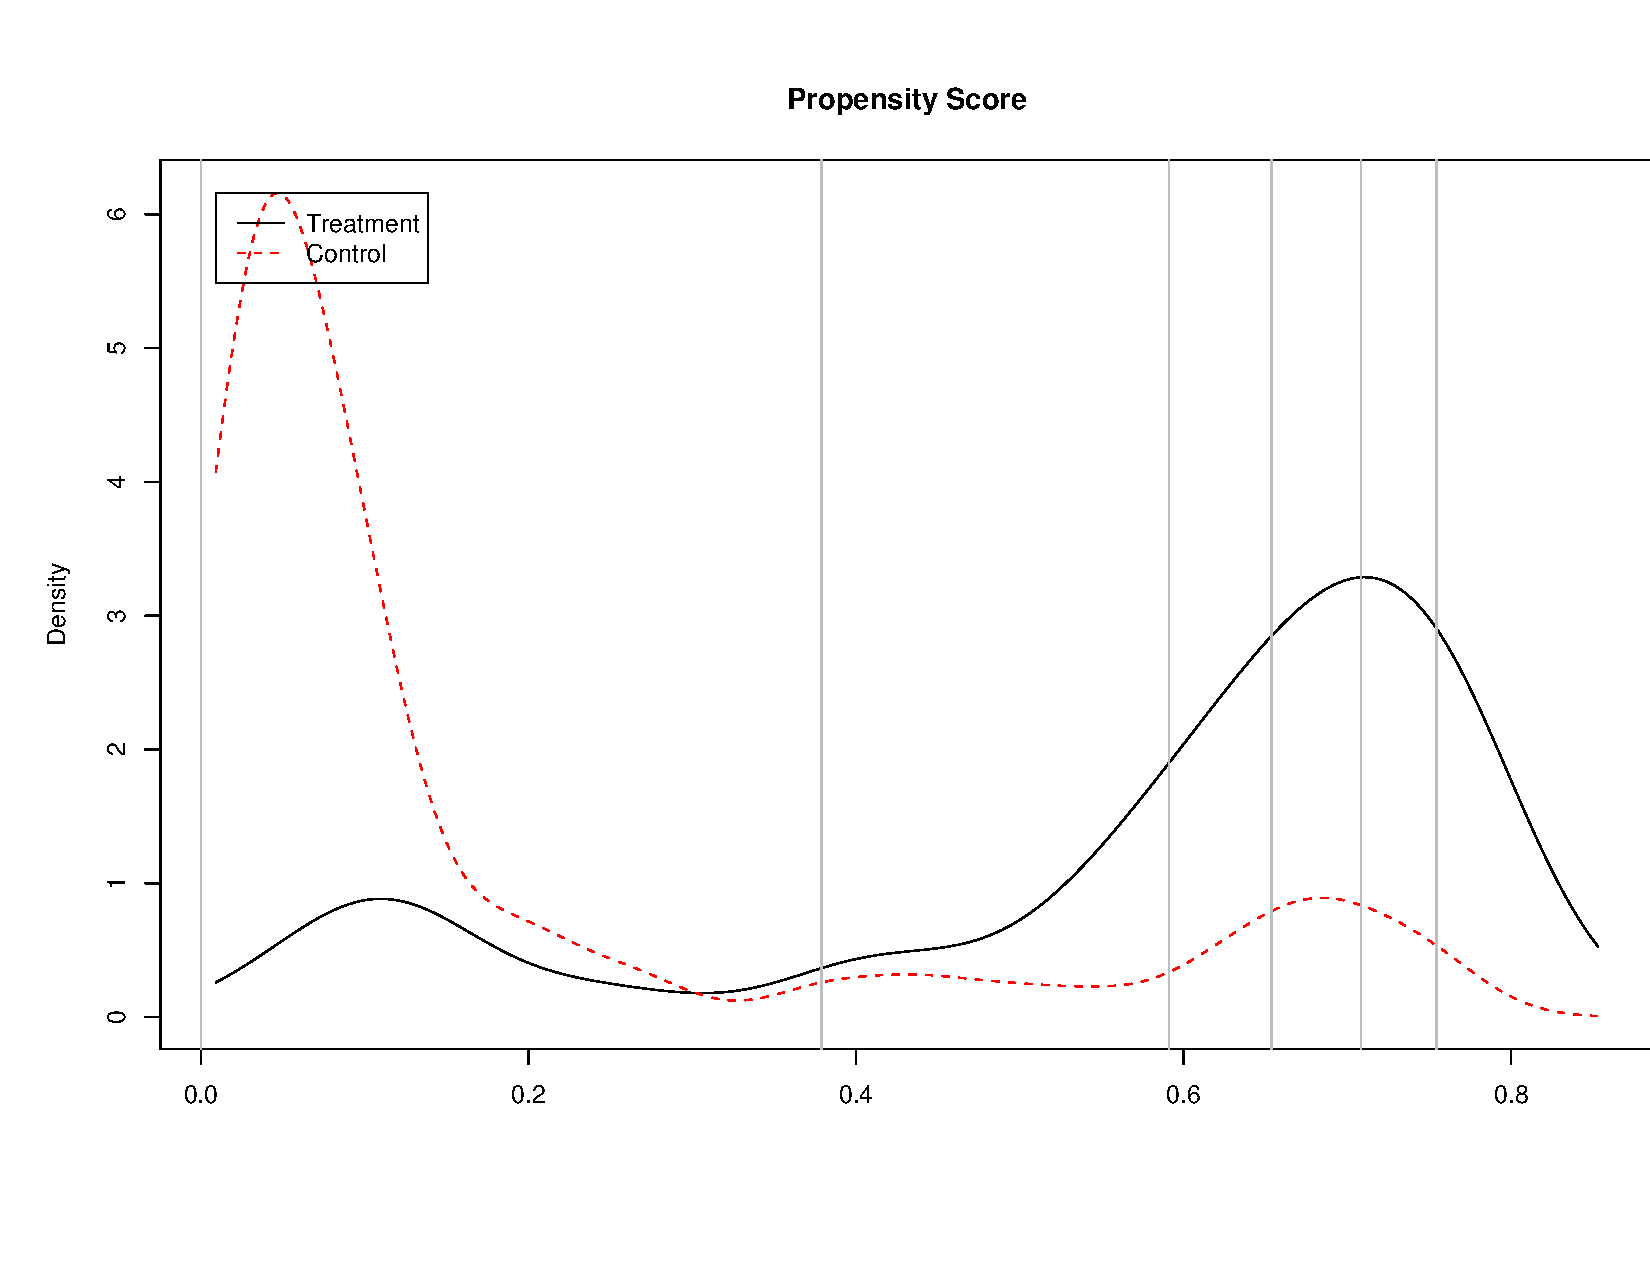
\includegraphics[height=2.85in,angle=0]{figs/subclass1}}
%    \rotatebox{270}{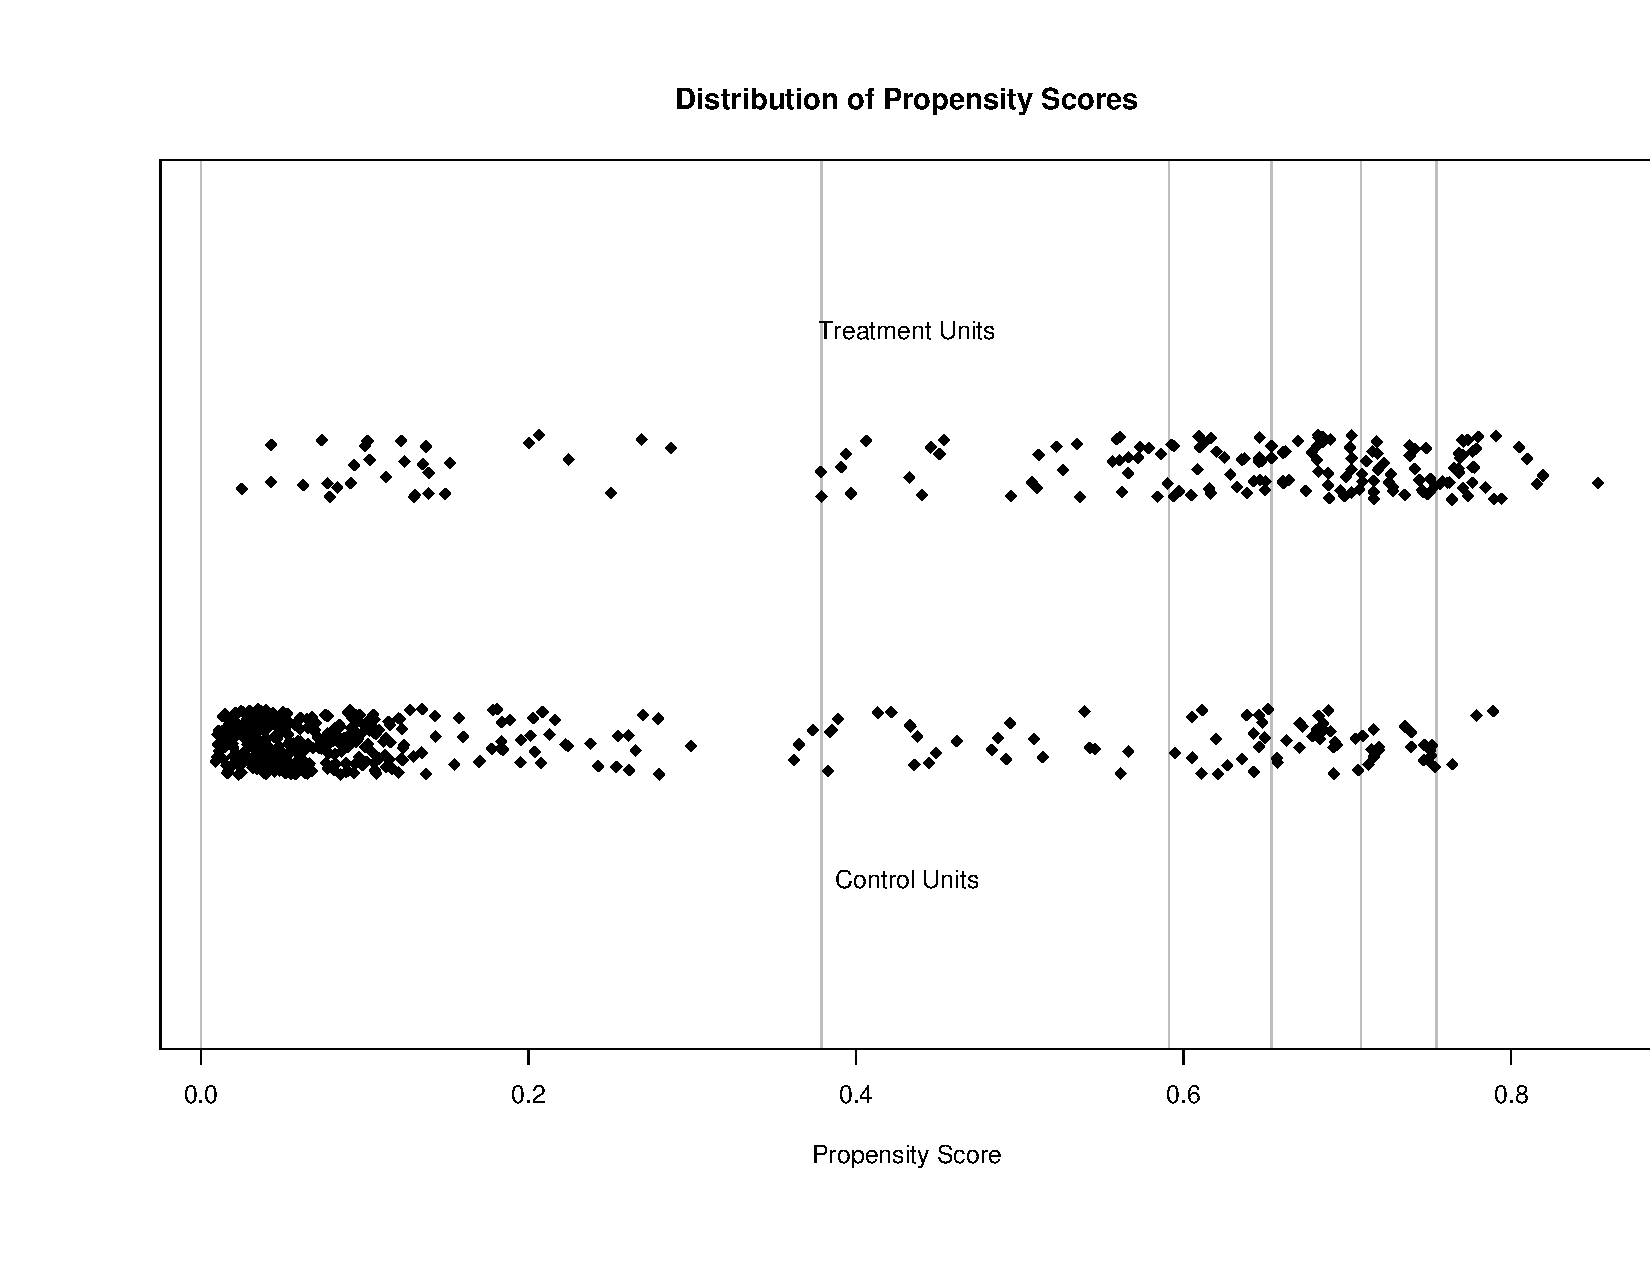
\includegraphics[height=2.85in,angle=0]{figs/subclass2}}
%    \rotatebox{270}{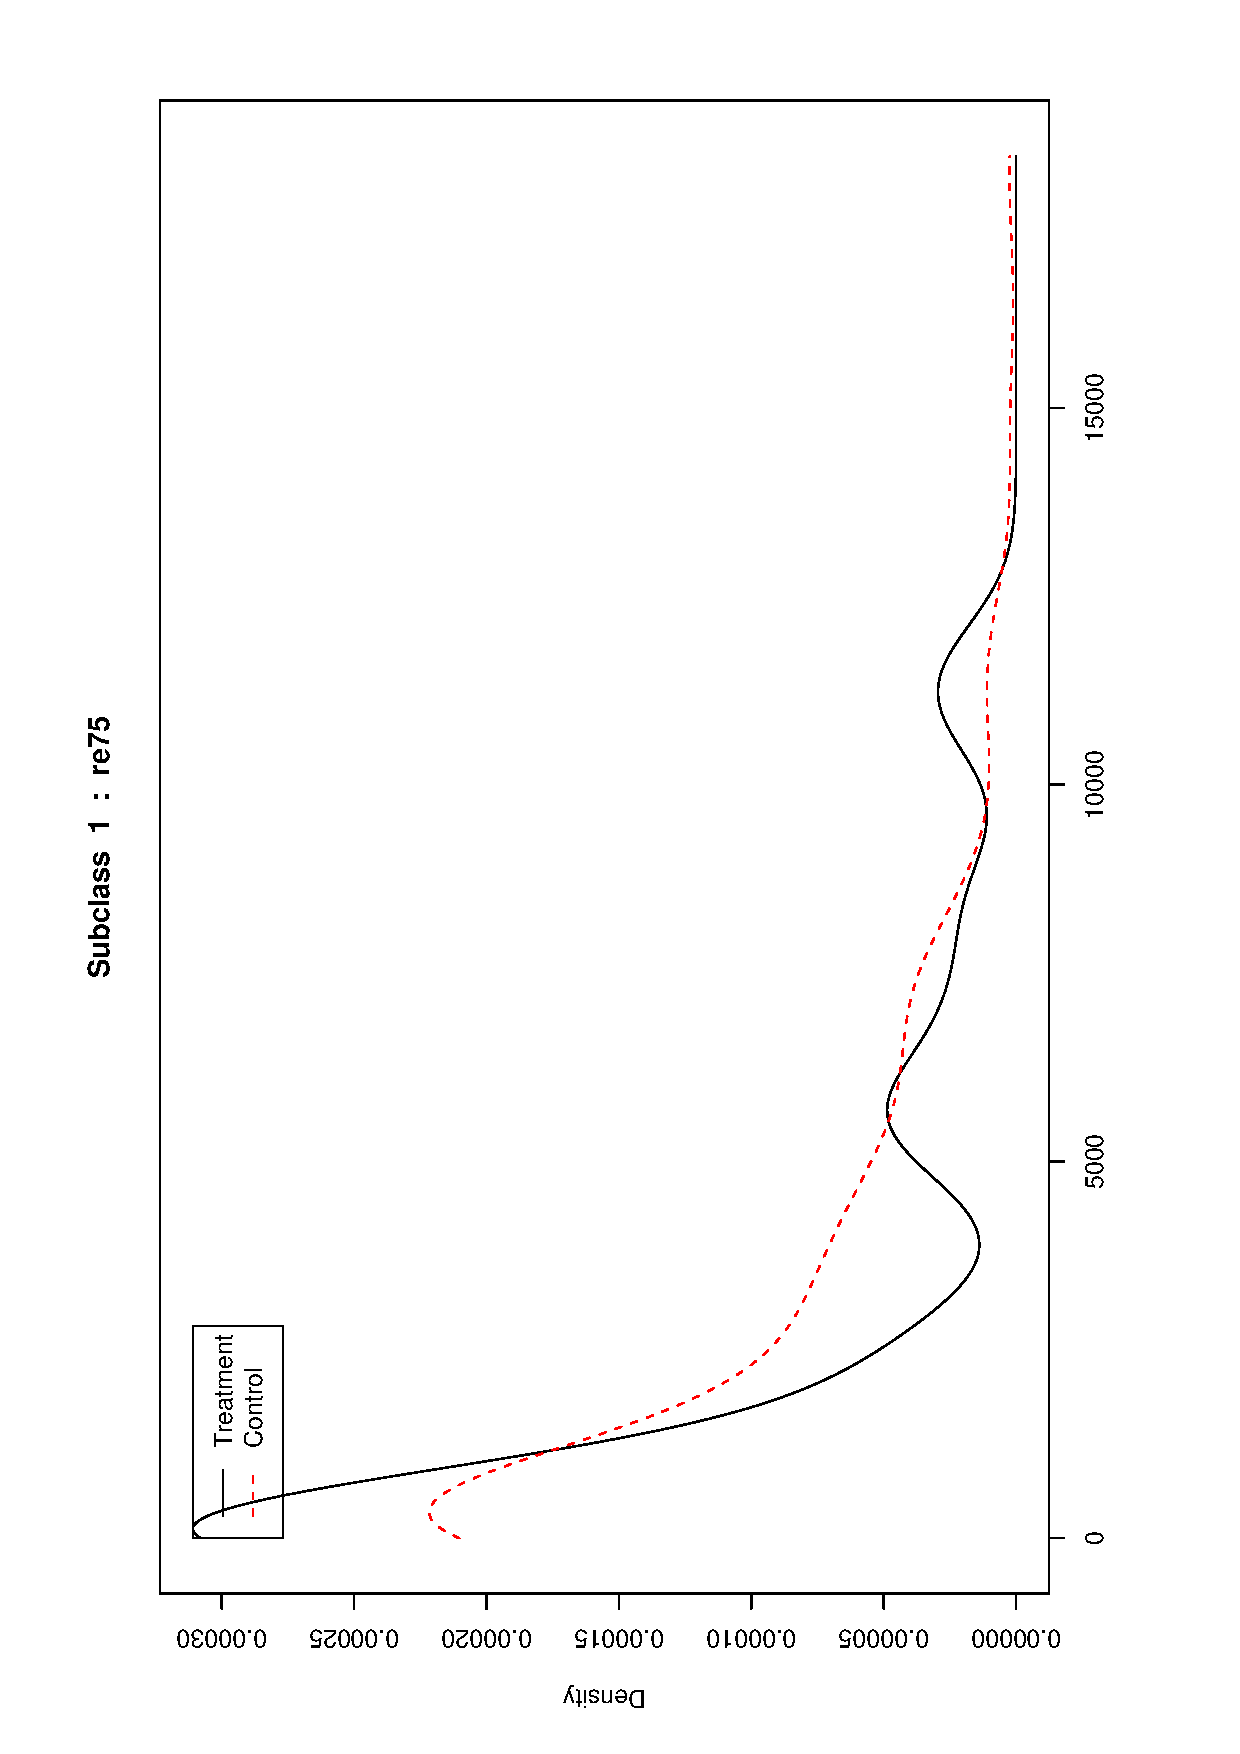
\includegraphics[height=2.85in,angle=0]{figs/subclass3}}
%    \rotatebox{270}{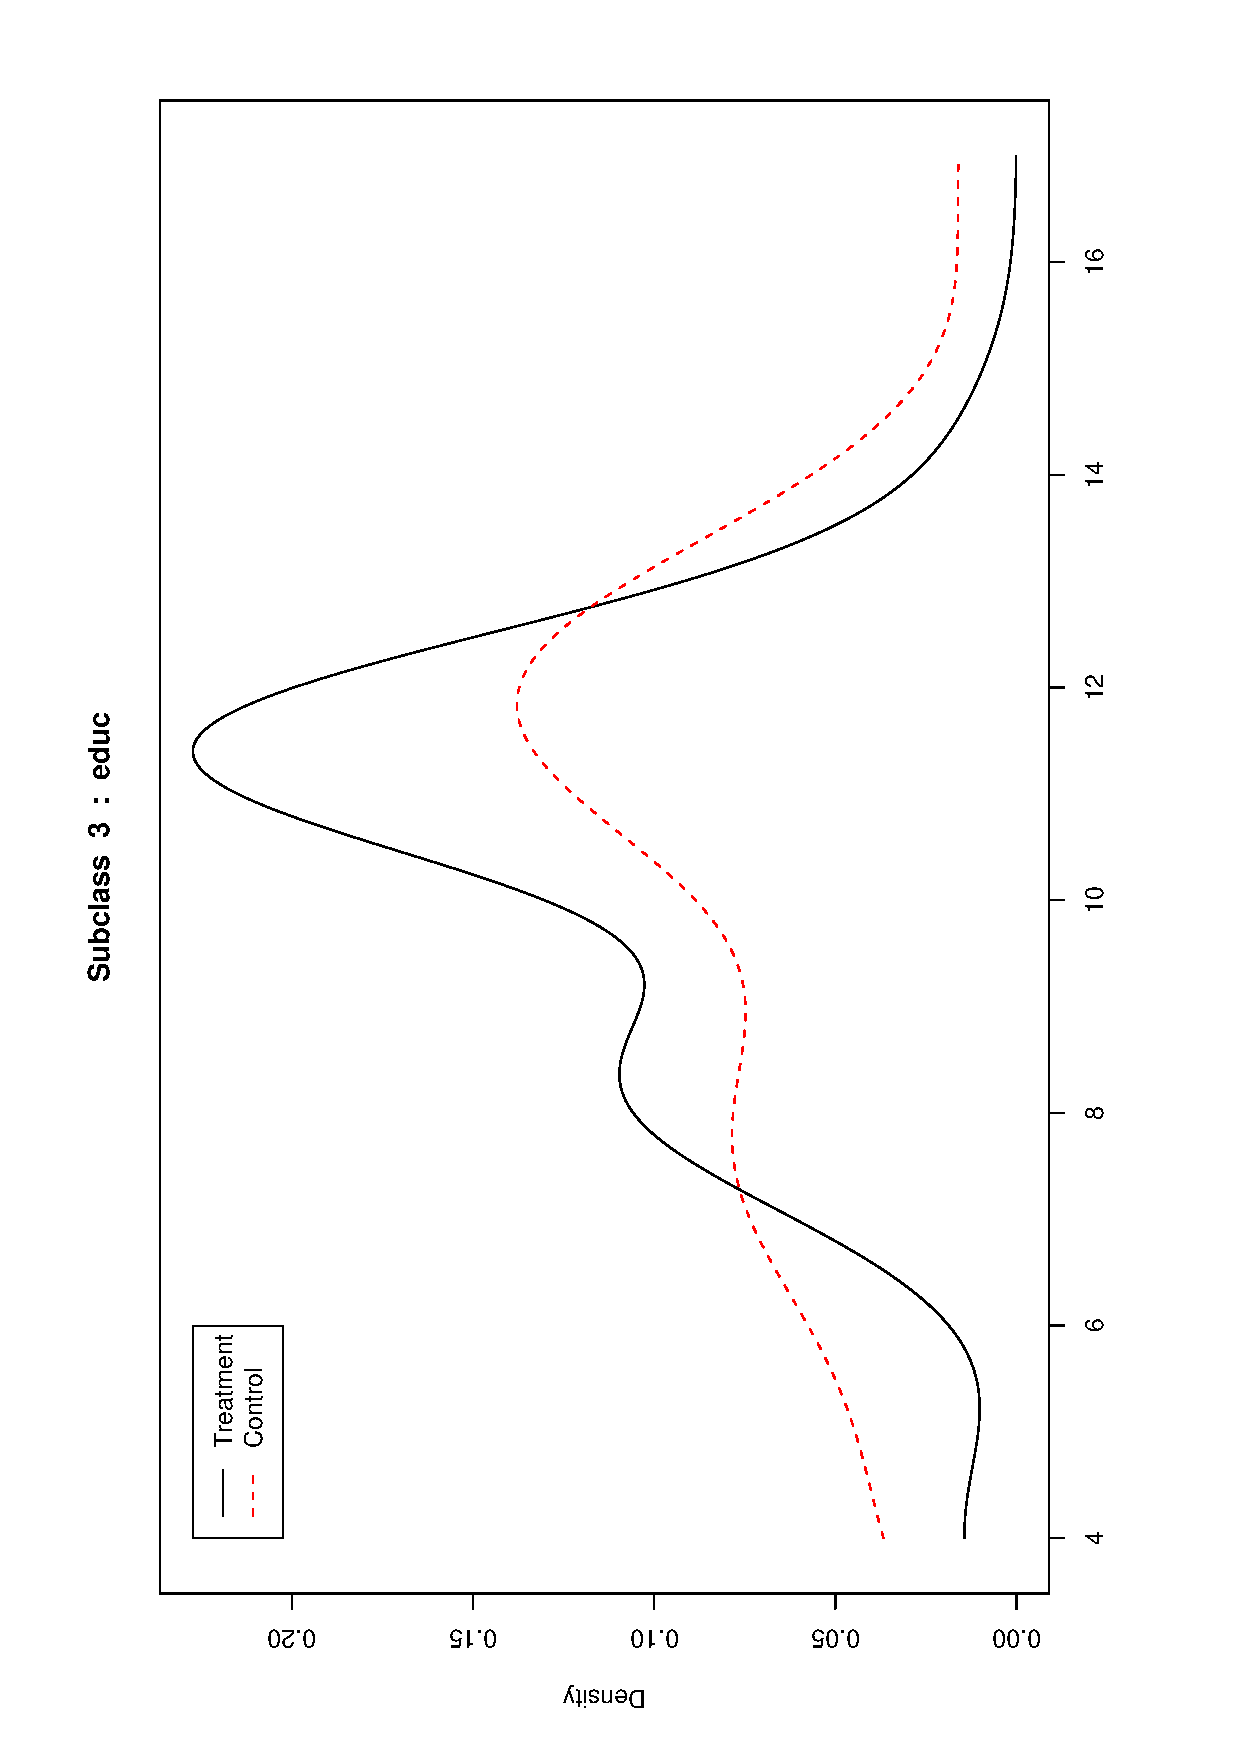
\includegraphics[height=2.85in,angle=0]{figs/subclass4}}
    {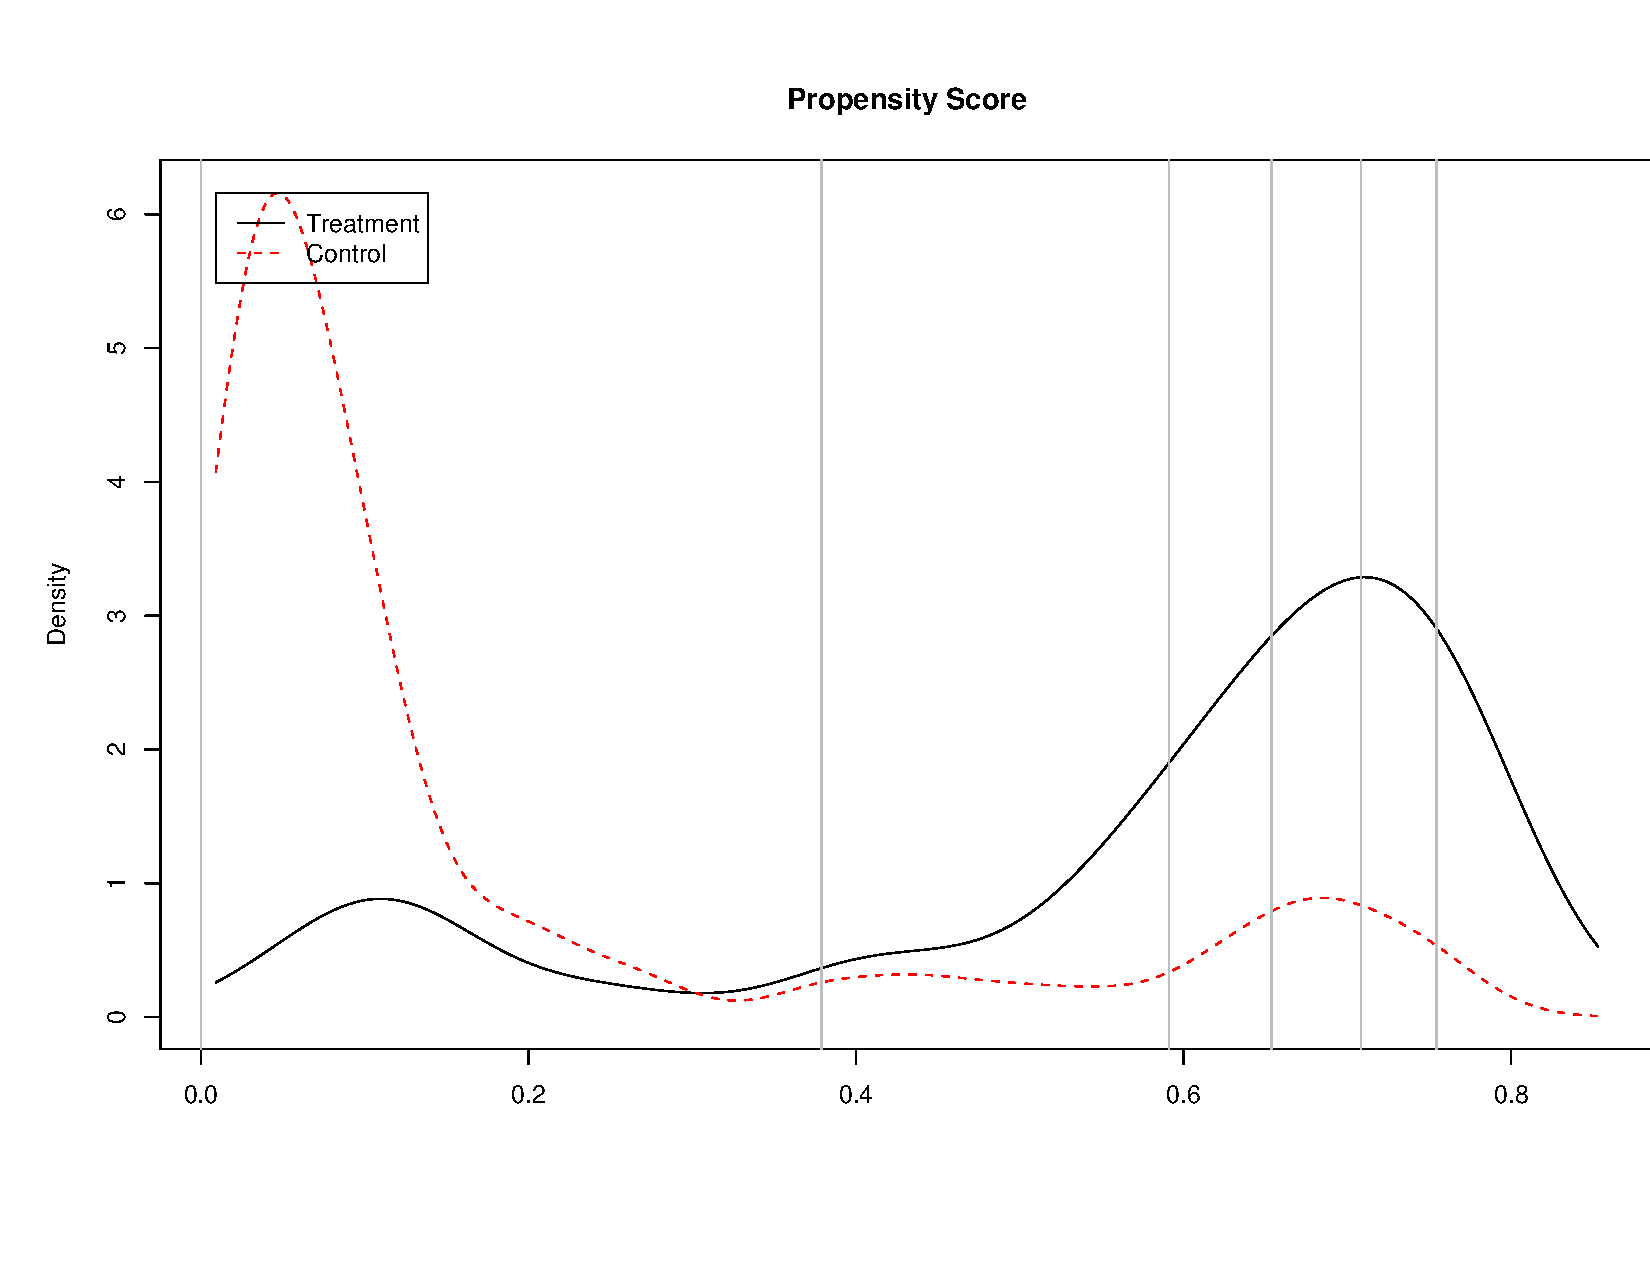
\includegraphics[scale=0.25]{figs/subclass1}}
    {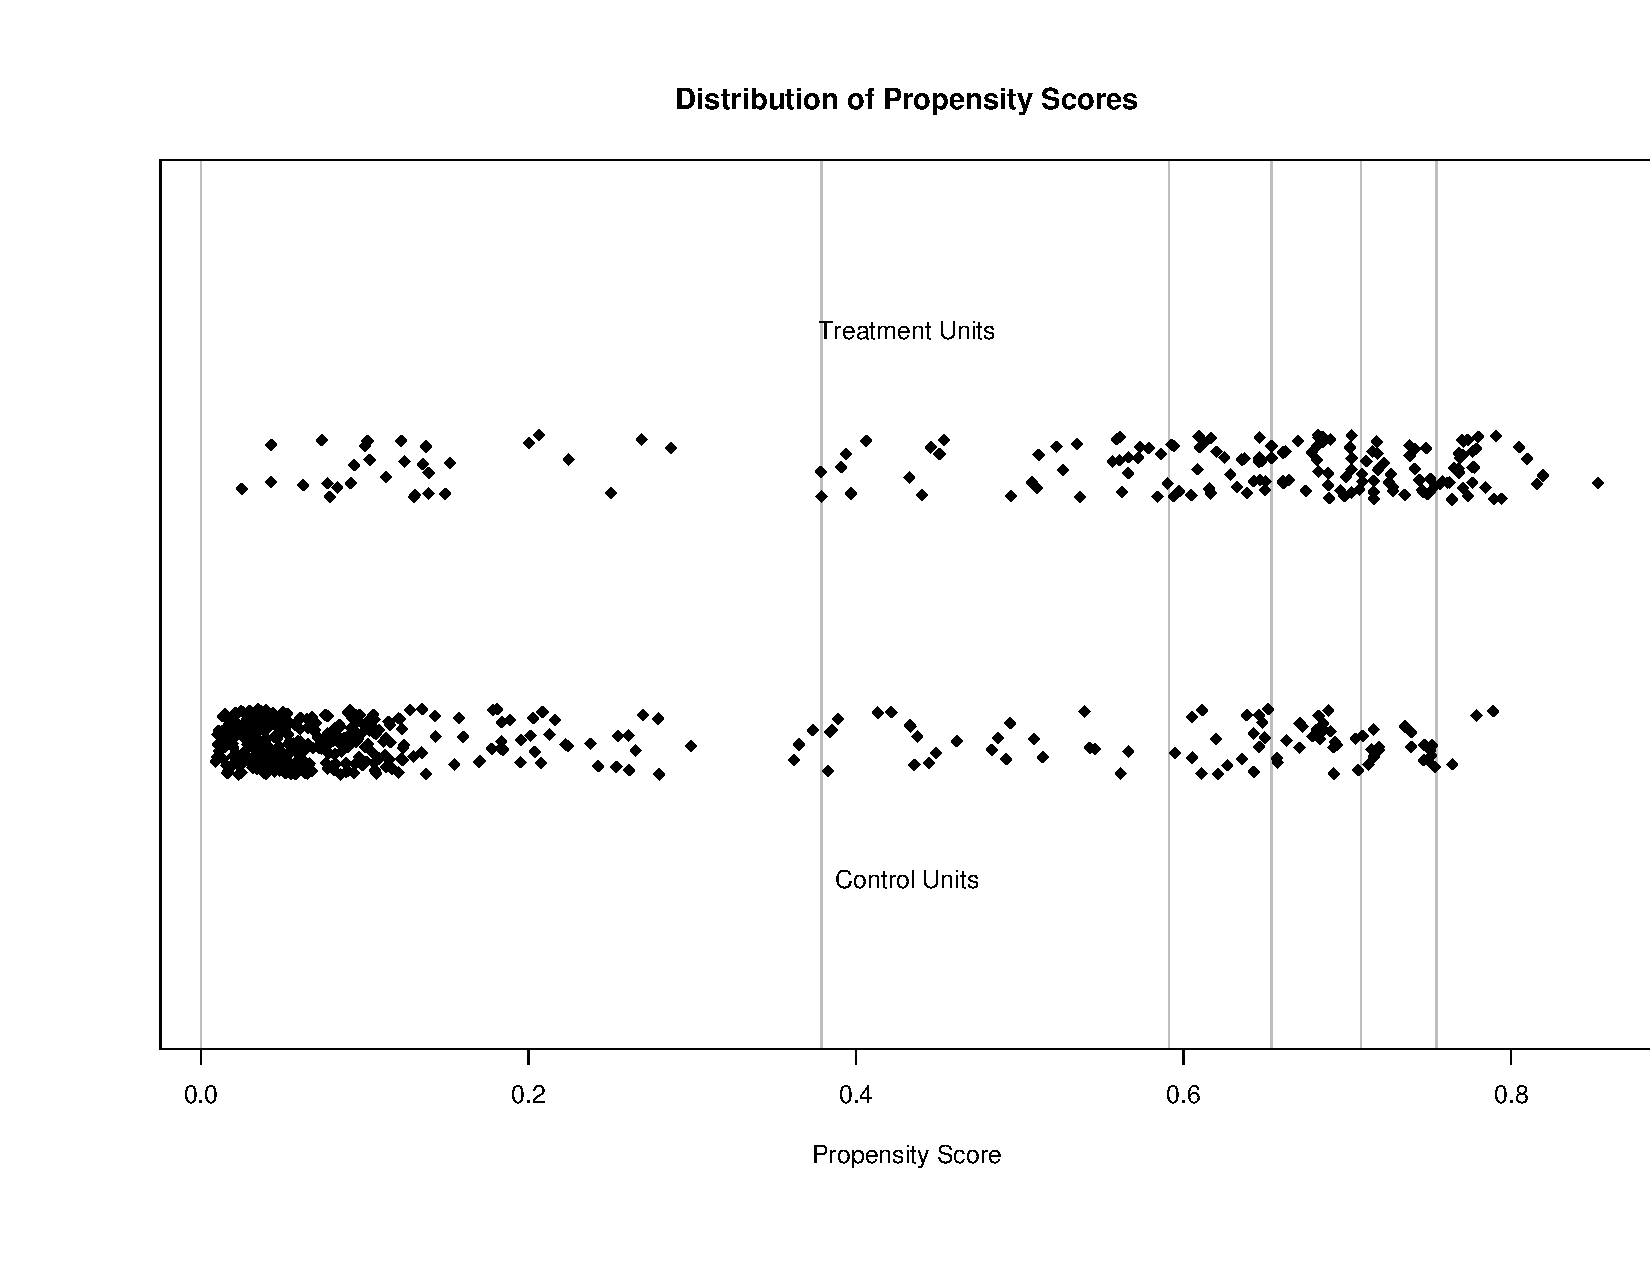
\includegraphics[scale=0.25]{figs/subclass2}}
    {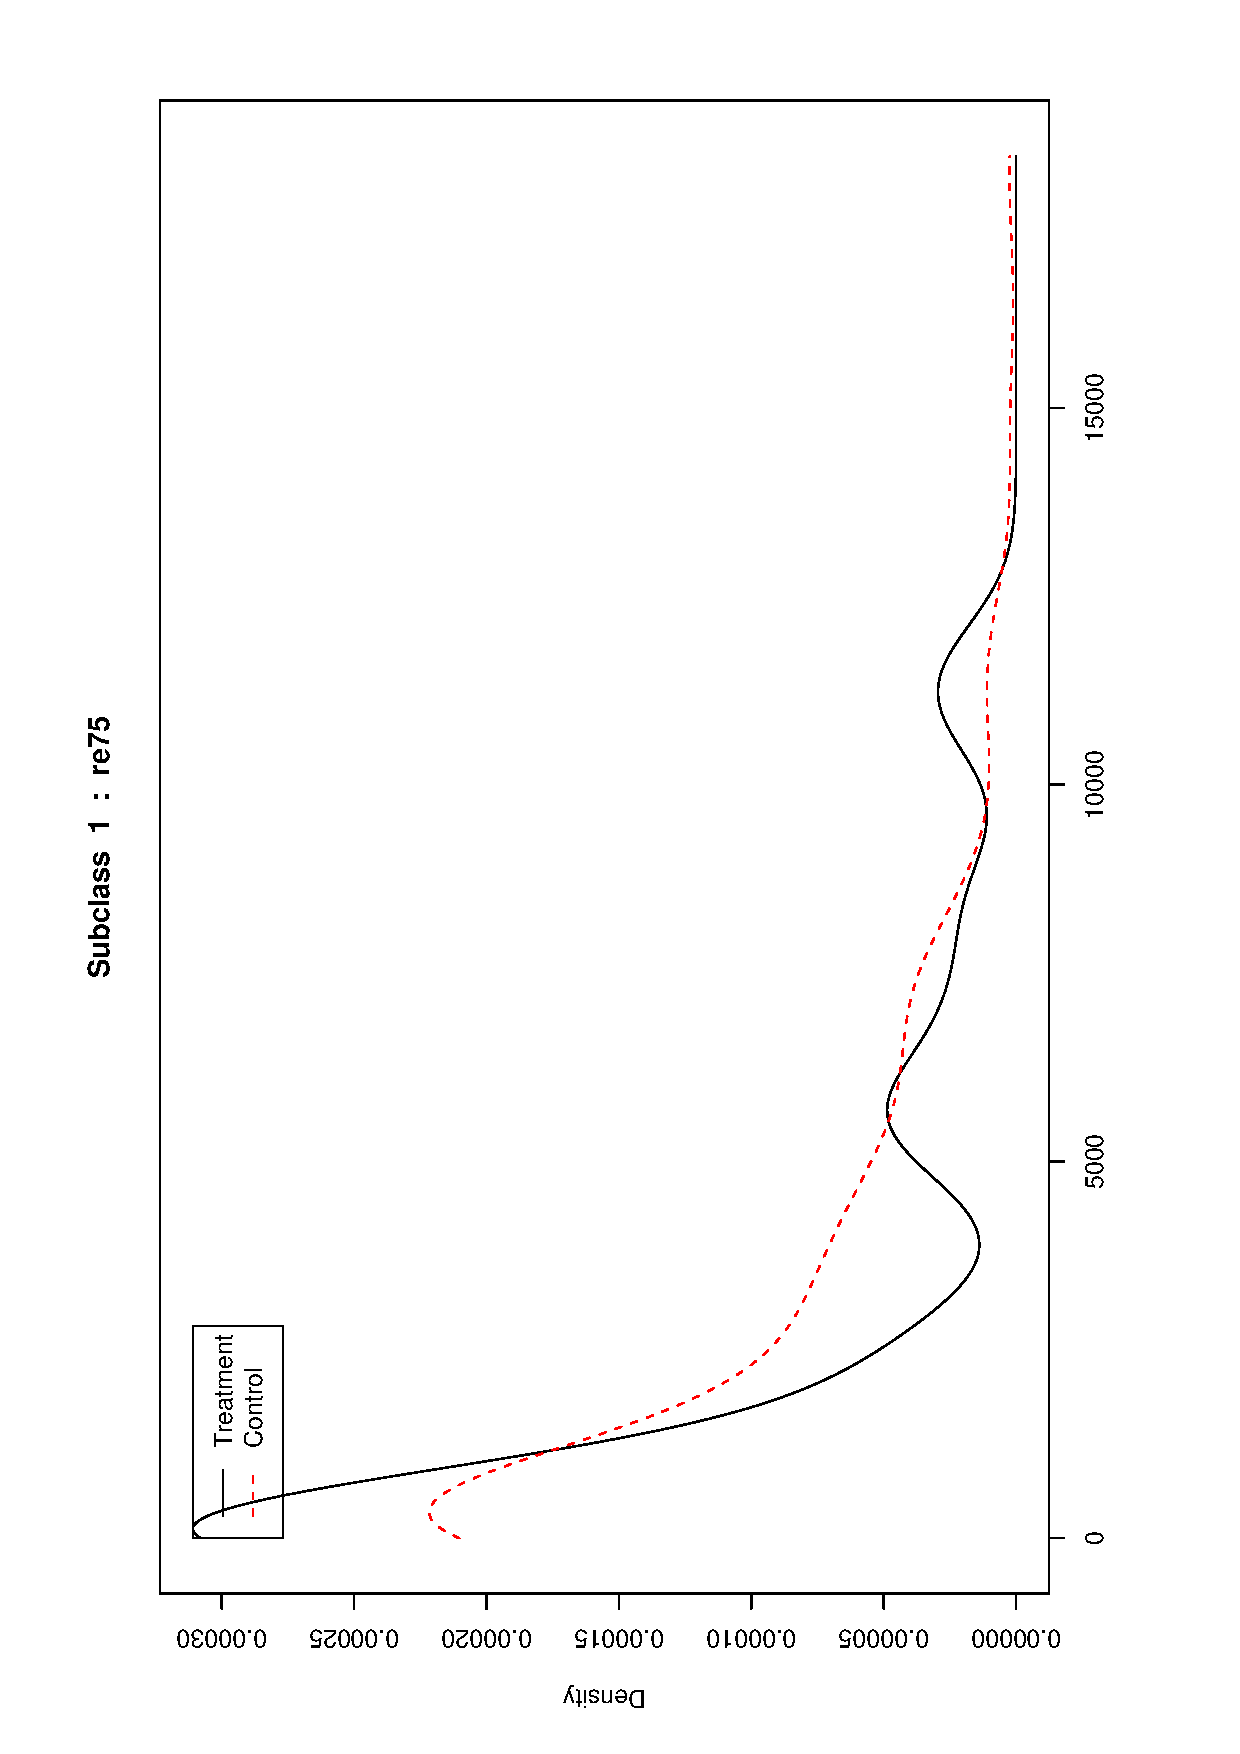
\includegraphics[scale=0.25,angle=90]{figs/subclass3}}
    {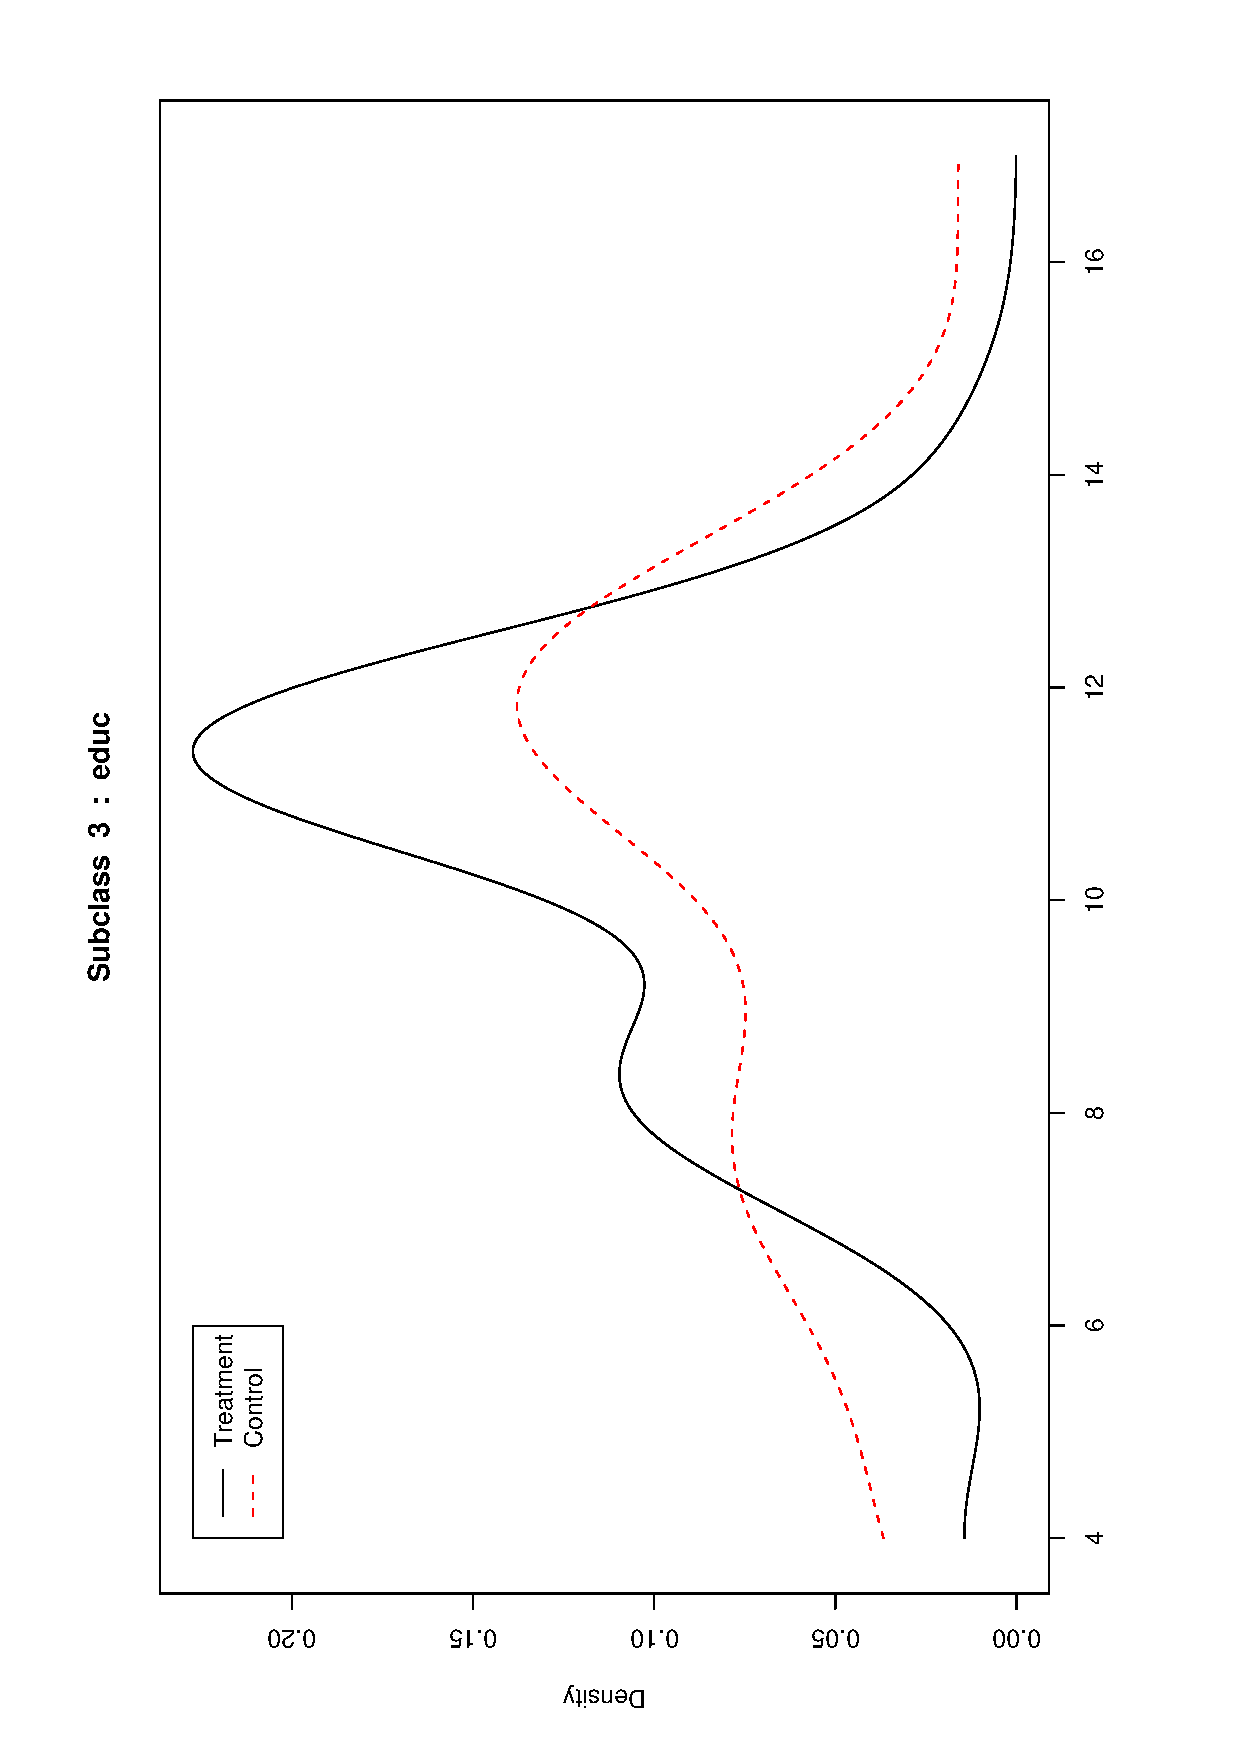
\includegraphics[scale=0.25]{figs/subclass4}}
    \hfill
    \caption{Sample interactive diagnostic graphs from \texttt{demo(lalonde)}}
\label{diags}
\end{center}
\end{figure}
\end{comment}

\subsection{Full Matching}
\label{fullmatching}

When one wishes to use all treated and control units in the analysis,
a particular type of subclassification is called ``full matching''
\citep{Rosenbaum02, Hansen04}. In this matching procedure, the matched
sample is composed of matched sets, where each matched set contains
either one treated unit and one or more controls, or one control unit
and one or more treated units.  Full matching is optimal in terms of
minimizing a weighted average of the propensity score distances
between each treated subject and each control subject within each
stratum.  

\subsubsection{Options}

Full matching can be performed with \MatchIt\ by setting
\texttt{method = "full"}.  We use an add-on package called
\texttt{optmatch} \citep{Hansen04}, which must be installed separately
by typing at the R command prompt,
\begin{verbatim}
> install.packages("optmatch", contriburl = "http://www.stat.lsa.umich.edu/~bbh/optmatch")
\end{verbatim}
Currently, \texttt{optmatch} is only available for Unix and MacOS X
(but not for Windows).  For more information about the package, see
\hlink{http://www.stat.lsa.umich.edu/\~{}bbh/optmatch.html}{http://www.stat.lsa.umich.edu/\~bbh/optmatch.html}.
The available options are listed below.

\begin{enumerate}
\item {\tt verbose} specifies whether some helpful comments are
  printed on the screen. The default is {\tt FALSE}
\item {\tt ...} represents additional inputs that can be passed to the
  {\tt fullmatch()} function in the {\tt optmatch} package. See {\tt
    help(fullmatch)} for details.
\end{enumerate}

\subsubsection{Examples}

The following example script can be run by typing {\tt demo(full)} at
the R prompt.

\begin{verbatim}
## load the Lalonde data
data(lalonde)
## conduct full matching using the propensity score based on logistic regression
m.out <- matchit(treat ~ age + educ + black + hispan + married + nodegree + re74 + re75, 
                 data = lalonde, method = "full", distance = "logit")
## print a short summary
print(m.out)
## balance diagnostics through statistics
summary(m.out)
## balance diagnostics through plots
plot(m.out)
\end{verbatim}


\subsection{Nearest Neighbor Matching}
\label{nearest}

Nearest neighbor matching selects the $r$ best matches for each
individual in the treatment group (excluding those discarded using the
\texttt{discard}) option.  The matching is done using a distance
measure such as the propensity score, and matches are chosen for each
treated unit one at a time, where at each step the control unit not
yet matched that is closest to the treated unit on the distance
measure is chosen as the match.  There are many variations on nearest
neighbor matching.  See below for the options available in /MatchIt/.

Nearest neighbor matching is implemented in /MatchIt/ using the
\texttt{method="nearest"} option.

\subsubsection{Options}
\begin{enumerate}
\item \texttt{m.order}  specifies the order in which to match
  treatment units with control units:
  \begin{itemize}
  \item {\tt "largest"} indicates matching from the largest value of
    the distance measure to the smallest. This is the default.
  \item {\tt "smallest"} indicates matching from the smallest value of
    the distance measure to the largest.
  \item {\tt "random"} indicates matching in random order.
  \end{itemize}
\item \texttt{ratio} specifies the number of control units to match to
  each treated unit, default=1.
\item \texttt{replace} specifies whether each control unit can be
  matched to more than one treated unit.  For matching ``with
  replacement'', \texttt{replace = TRUE}.  If each control is to be
  used as a match only once (``without replacement''), \texttt{replace
    = FALSE}. The default is {\tt FALSE}.
\item \texttt{exact} specifies variables on which to perform exact
  matching within the nearest neighbor matching.  If \texttt{exact} is
  specified, only matches that exactly match on the covariates in
  \texttt{exact} will be selected.  Within the matches that match on
  the variables in \texttt{exact}, the match with the closest distance
  measure will be chosen.  \texttt{exact} should be entered as a
  vector of variable names \texttt{exact = c("X1", "X2")} that are
  names of variables in \texttt{data}.
\item \texttt{caliper} specifies the number of standard deviations of
  the distance measure within which to draw control units, default=0.
  If a caliper is specified, the matches are restricted to being
  within the caliper and a control unit within the caliper for a
  treated unit is randomly selected as the match for that treated
  unit.  If \texttt{caliper != 0}:
  \begin{itemize} 
  \item \texttt{calclosest} specifies whether to take the nearest
    available match if no matches are available within
    \texttt{caliper}. The default is {\tt FALSE}.
  \item \texttt{mahvars} specifies variables on which to perform
    Mahalanobis-metric matching within each caliper (default=NULL).
    Variables should be entered as a vector of variable names
    \texttt{mahvars=c("X1","X2")} that are names of variables in
    \texttt{data}.  If \texttt{mahvars} is specified without
    \texttt{caliper}, the caliper is set to 0.25.
  \end{itemize}
\item \texttt{subclass} and \texttt{sub.by}.  See Section
  \ref{subclass} for more details on these options.  If a
  \texttt{subclass} is specified within \texttt{method = "nearest"},
  subclasses will be formed using the matched units after the nearest
  neighbor matching is completed.
\end{enumerate}

Ratio matching with a ratio greater than 1 is sometimes used to
increase efficiency of the estimand when there is a large number of
comparable control units available. If matching is done without
replacement and there are fewer control units than ratio times the
number of eligible treated units (i.e., there are not enough control
units for the specified method), then the higher ratios will have
\texttt{NA} in place of the matching unit number in
\texttt{match.matrix}.

\subsubsection{Examples}

\begin{enumerate}
\item The following example script can be run by typing {\tt
    demo(nearest)} at the R prompt.

\begin{verbatim}
## load the Lalonde data
data(lalonde)
## Nearest neighbor matching on propensity score estimated using logistic regression of
## treat on re74, re75, age, and educ.  Two matches chosen for each control unit.
m.out <- matchit(treat ~ re74 + re75 + age + educ, data = lalonde, method = "nearest", 
                 distance = "logit", ratio=2)
## print a short summary
print(m.out)
## print out summary of balance in matched samples
summary(m.out)

## Mahalanobis matching on re74 and re75 within nearest neighbor matching on 
## distance measure, with restriction of exact matches on married.
m.out2 <- matchit(treat ~ re74 + re75 + age + educ, data = lalonde, method = "nearest", 
                  distance = "logit", mahvars=c("re74", "re75"), exact=c("married"), 
                  caliper=.25)
print(m.out2)
summary(m.out2)

## Nearest neighbor matching with discard option
m.out3 <- matchit(treat ~ re74 + re75 + age + educ, data = lalonde, method = "nearest", 
                  distance = "logit", discard="both")
print(m.out3)
summary(m.out3)

## Nearest neighbor matching with replacement
m.out4 <- matchit(treat ~ re74 + re75 + age + educ, data = lalonde, method = "nearest", 
                  distance = "logit", replace=TRUE, ratio=2)
print(m.out4)
summary(m.out4)

## Nearest neighbor matching followed by formation of 5 subclasses
m.out5 <- matchit(treat ~ re74 + re75 + age + educ, data = lalonde, method = "nearest", 
                  distance = "logit", subclass=5)
print(m.out5)
summary(m.out5)
\end{verbatim}

\item We can examine which units were matched to which using the {\tt
    match.matrix} output:
\begin{verbatim}
> foo3$match.matrix
            V1
NSW1   PSID406
NSW2   PSID385
NSW3   PSID388
NSW4   PSID326
NSW5   PSID337
NSW6   PSID376
NSW7   PSID134
NSW8   PSID355
NSW9      <NA>
NSW10  PSID422
...  
\end{verbatim}  

The unit numbers on the left are the treated units; the units in the
2nd column are the controls matched to each treated unit.  For
example, PSID Unit 406 was matched to NSW Unit 1.  NSW Unit 9 did not
have a match.  We can verify that the matched pairs have identical
race values (\texttt{black} and \texttt{hispan}):

\begin{verbatim}
> lalonde[c("NSW1", "PSID406"), c("black", "hispan")]
        black hispan
NSW1        1      0
PSID406     1      0

> lalonde[c("NSW2", "PSID385"), c("black", "hispan")]
        black hispan
NSW2        0      1
PSID385     0      1
\end{verbatim}


\item Replication of \citet{DehWah99}. The following line replicates
  the matching algorithm of Table 2 (column 10, row 4):

\begin{verbatim}
## load the Lalonde data
data(lalonde)           
## matching with replacement     
foo <- matchit(treat ~ age + I(age^2) + educ + I(educ^2) + black +
               hispan + married + nodegree + re74 + I(re74^2) + re75 + I(re75^2) +
               I(as.numeric(re74==0)) + I(as.numeric(re75==0)), data=lalonde,
               replace = TRUE, discard = "both")
\end{verbatim}

  Note that the only differences between this and the earlier
  propensity score matching example are: (a) the number of covariates
  used, (b) the \texttt{discard} option (which drops control units
  outside the support of the treated group's propensity scores, and
  (c) matching with replacement (so that each control unit can be
  matched to more than one treated unit).
\end{enumerate}

\subsection{Optimal Matching}
\label{optmatch}

The default nearest neighbor matching method in \MatchIt\ is
``greedy'' matching, where the closest control match for each treated
unit is chosen one at a time, without trying to minimize a global
distance measure.  Another method, ``optimal'' matching, finds the
matched samples with the smallest average absolute propensity score
distance between each matched pair.  With large control pools, greedy
and optimal matching may lead to very similar (or the same) sets of
matches; research \citep{GuRos93} has shown that greedy and optimal
matching generally choose the same sets of controls for the matched
samples, but that optimal matching does a better job of minimizing the
propensity score distance within each pair.  In addition, optimal
matching can be particularly helpful when there are not many
appropriate control matches for the treated units.  See \cite{GuRos93}
or \cite{Rosenbaum02} for more information on optimal matching.

\subsubsection{Options}

Optimal matching can be performed with \MatchIt\ by setting
\texttt{method = "optimal"}.  We use an add-on package called
\texttt{optmatch} \citep{Hansen04}, which must be installed separately
by typing at the R command prompt,
\begin{verbatim}
> install.packages("optmatch", contriburl = "http://www.stat.lsa.umich.edu/~bbh/optmatch")
\end{verbatim}
Currently, \texttt{optmatch} is only available for Unix and MacOS X
(but not for Windows).  For more information about the package, see
\hlink{http://www.stat.lsa.umich.edu/\~{}bbh/optmatch.html}{http://www.stat.lsa.umich.edu/\~bbh/optmatch.html}.
The available options are listed below.

\begin{enumerate}
\item {\tt ratio} specifies the the number of control units to be
  matched to each treatment unit, the default is {\tt 1}.
\item {\tt verbose} specifies whether some helpful comments are
  printed on the screen. The default is {\tt FALSE}
\item {\tt ...} represents additional inputs that can be passed to the
  {\tt fullmatch()} function in the {\tt optmatch} package. See {\tt
    help(fullmatch)} for details.
\end{enumerate}

\subsubsection{Examples}

The following example script can be run by typing {\tt demo(optimal)}
at the R prompt.

\begin{verbatim}
## load the Lalonde data
data(lalonde)
## optimal ratio matching using the propensity score based on logistic regression
m.out <- matchit(treat ~ re74 + re75 + age + educ, data = lalonde, method = "optimal", 
                 distance = "logit", ratio = 2)
## a short summary
print(m.out)
## balance diagnostics through statistics
summary(m.out)
## balance diagnostics through graphics
plot(m.out)
\end{verbatim}


\subsection{Balance Diagnostics}
\label{pscorespec}

\subsubsection{Options}

\subsubsection{Examples}

The model specification and diagnostics for propensity scores are not
the standard model diagnostics for logistic regression or CART.  With
propensity score estimation, and matching methods more generally,
concern is not with the parameter estimates of the model (after all,
the outcome variable is not even used in the matching procedure), but
rather with the quality of the matches.  Because matching does not
make use of the outcome values, and the subsequent parametric analysis
is conditional on all the variables used in the matching procedure,
matching can be done multiple times and the best matched sample chosen
without biasing causal estimates from the ultimate parametric
analysis.  Diagnostics for propensity scores thus involve assessing
specifications and choosing the single specification with the best
balance between the matched treated and control groups.  If covariates
(or their squares or cross-products) are found to be imbalanced, those
terms are then included in the propensity score specification, which
should improve their balance.  

A sample strategy is described here:

\begin{enumerate}
\item Start with a model (for example, logistic regression with the
  treatment as the response variable) with main effects for each of
  the observed covariates.  The propensity scores are the predicted
  probabilities of treatment assignment generated from the model
  conditional on the observed covariates.
\item Possibly discard control units outside the range of the treated
  group propensity scores, and/or treated units outside the range of
  the control group propensity scores.  This eliminates nonrobust
  extrapolation but changes the quantity being estimated.
\item Form 2 subclasses (with propensity scores split at their
  median), do a t-test of the propensity score in the treated and
  control groups in each subclass.  If there is a significant
  difference, split each subclass into 2 subclasses at its median.
  Continue this process, splitting a subclass if it has a t-statistic
  greater than 2.5 and if there are two or more treated and control
  units in each new subclass formed.
\item Within each subclass formed in Step 3, test for equality of
  means of functions of X (e.g., each covariate, each covariate
  squared, 2-way interactions of covariates).  If any t-statistic is
  greater than 2 in any subclass, include that term in the new
  propensity score specification.  (Other, similar rules can be used,
  such as including terms that are significant in more than 1
  subclass).
\item Repeat Steps 1-4 until there are no more (or very few, as few as
  possible) significant t-statistics.  This will imply that within
  each block the treated and control groups are very well balanced.
\end{enumerate}

This method can be implemented in \MatchIt\ in the following way.
First, run a propensity score model with main effects for each of the
covariates, first with just two subclasses, divided at the median
propensity score:

\begin{verbatim}
> match.out1 <- matchit(treat ~ age + married + black + hispan +
                      nodegree + educ + re74 + re75, data=lalonde,                      
                      subclass=c(0, .5, 1))

> summary(match.out1, verbose=F)
\end{verbatim}

The following is an excerpt from the output:

\begin{verbatim}
, , Subclass 1

         means.t.q means.c.q    sd.q    t.q bias.q reduction.q
pscore        0.42      0.26    0.22   5.71   0.55           1
Number       91.00    143.00  234.00 234.00 234.00         234

, , Subclass 2

         means.t.q means.c.q    sd.q    t.q bias.q reduction.q
pscore        0.73      0.71    0.04   2.68   0.06           1
Number       94.00     42.00  136.00 136.00 136.00         136

Problematic covariates:
Subclass  1 :  pscore black hispan
Subclass  2 :  pscore
Number of units discarded:   0

\end{verbatim}

Because the t-statistics of the propensity scores in both subclasses
are greater than 2.5, we divide each block in half, at its median:

\begin{verbatim}
> match.out1 <- matchit(treat ~ age + married + black + hispan +
                      nodegree + educ + re74 + re75, data=lalonde,                      
                      subclass=c(0, .25, .5, .75, 1))

> summary(match.out1, verbose=T)
\end{verbatim}

Because Subclass 4 still has a t-statistic greater than 2.5, we again
divide that subclass in half, leading to five subclasses.  All five
subclasses have t-statistics of the propensity score less than 2.5.
We then run {\tt summary(match.out1, verbose=T)} on that matchit
object, to examine the balance of all of the squares and interactions
of the covariates within each subclass.

\begin{verbatim}
> match.out1 <- matchit(treat ~ age + married + black + hispan +
+                       nodegree + educ + re74 + re75, data=lalonde,
+                       subclass=c(0, .25, .5, .75,.875, 1))
Calculating propensity score...Done
Matching Treated: 10%...20%...30%...40%...50%...60%...70%...80%...90%...100%...Done
Subclassifying...Done
Calculating summary statistics...Done
> summary(match.out1, verbose=T)
\end{verbatim}

We are interested in the ``Problematic covariates.''  For subclasses,
this is a list of all covariates, squares, and two-way interactions
that have t-statistics greater than $2$ in any subclass (the default
of $2$ can be changed by specifying the \texttt{sig} option in the
{\texttt summary} command).

\begin{verbatim}
Problematic covariates:
Subclass  1 :  black re74 blackxblack blackxeduc blackxre74
Subclass  2 :  married agexmarried marriedxmarried marriedxblack marriedxnodegree 
               marriedxeduc nodegreexeduc
Subclass  3 :  
Subclass  4 :  agexnodegree
Subclass  5 :  
\end{verbatim}

These ``problematic'' covariates are then included in the new
propensity score specification, and the process is repeated.  (Note:
since {\tt black} and {\tt married} are binary covariates, their
squares are just the variables themselves and thus the squares are not
included in the new specification.)

\begin{verbatim}
> match.out2 <- matchit(treat ~ age + educ + married + nodegree + hispan +
                      black + re74 + re75 + I(black*educ) +
                      I(black*re74) + I(age*married) + I(married*black) + 
                      I(married*nodegree) + I(married*educ) +
                      I(nodegree*educ) + I(age*nodegree),
                      data=lalonde, subclass=c(0,.5,1))

> summary(match.out2, verbose=F)
\end{verbatim}

This process leads to three blocks being created  ({\tt subclass=c(0, .25, .5, 1)}).

\begin{verbatim}
> match.out2 <- matchit(treat ~ age + educ + married + nodegree + hispan
                      + black + re74 + re75 + I(educ*black) +
                      I(black*re74) + I(age*married) + I(educ*married)
                      + I(educ*nodegree) + I(married*nodegree) +
                      I(married*black) + I(age*nodegree),
                      data=lalonde, subclass=c(0,.25,.5,1))

> summary(match.out2, verbose=F)
\end{verbatim}

We see that now there are only 2 ``problematic covariates,'' in just
one subclass.  We use {\tt verbose=F} at this stage so that we are
checking just the balance of the squares and two-way interactions of
the covariates themselves; {\tt verbose=T} here would give details on
the squares and interactions of the interaction variables, which are
generally not of as much interest as the two-way interactions
themselves.  Because good balance has been achieved and the two
problematic covariates are already included, we stop here and use this
propensity score model, with the chosen interactions.

\begin{verbatim}
Problematic covariates:
Subclass  1 :  
Subclass  2 :  re74 I(black * re74)
Subclass  3 :  
\end{verbatim}

This section has provided one example of a diagnostic procedure for
propensity score models.  The details may vary (for example, an option
could be to include only squares and interactions that have a
significant difference in more than one block.)  The user could also
identify a different cut-point for the subclasses, or for significance
(as opposed to 2.5 and 2).

%%%%%%%%%%%%%%%%%%%%%%%%%%%%%%%%%%%%%%%%%%%%%%%%%%%%%%%%%%%%%%%%%%%%%%%%%%%
\clearpage

\section{Statistical Analysis after Matching}
\label{sec:analysis}

Once the matching is complete, the \MatchIt\ object can be used with
any other analysis procedure; \MatchIt\ is designed to make those
analysis procedures less dependent on the modeling assumptions and
thus work better.  Thus, any analysis you might have done using the
original data sets can be done better on the matched data sets.  To
obtain the matched data sets, use {\tt match.data(m.out)}, where {\tt
  m.out} is a \MatchIt\ object. See Section~\ref{subsec:match.data}
for more options and details.

In this section, we describe two possible analysis methods to use with
\MatchIt. First, we descibe a simple difference-in-means approach to
estimate the average treatment effect. Next, we descibe our
recommended approach \citep{HoImaKin05}, which uses
\hlink{Zelig}{http://gking.harvard.edu/zelig/} to conduct parametric
causal inference after preprocessing the data through \MatchIt.

\subsection{Using Neyman's Method to Estimate Average Treatment Effect}

{\tt neyman()} is a \MatchIt\ function which calculates a simple
difference in means and corresponding variance estimate.  For any more
sophisticated analyses (and even this simple case if you desire), we
recommend using \hlink{Zelig}{http://gking.harvard.edu/zelig/}, to
conduct a model-based analysis after matching. See
Section~\ref{subsec:Zelig} for more details.

\subsubsection{Estimation Details}

The estimated treatment effect is:
\begin{equation}
\label{ate} 
\widehat{ate} = \overline{y}_{mt}^w-\overline{y}_{mc}^w,
\end{equation}
where $\overline{y}_a^w$ is the weighted mean of the outcome in group
$a$ ($mt$ refers to the matched treated group, and $mc$ refers to the
matched control group).  The weighted mean is calculated as:
$$\overline{y}_a^w = \frac{\sum_{i=1}^n w_i y_i}{\sum_{i=1}^n w_i},$$
where $y_i$ is the outcome and $w_i$ is the weight for individual $i$
({\tt psweights} from the \MatchIt\ object).

The estimated variance of the estimated treatment effect in Equation
\eqref{ate} is:
\begin{equation}
\label{estvar}
\widehat{{\rm var}}(\widehat{ate}) = \frac{s_{mt}^2}{\sum_{i=1}^{n_1} w_i} + \frac{s_{mc}^2}{\sum_{i=1}^{n_0} w_i},
\end{equation}
where $s_a^2$ is the weighted variance of the outcome in group $a$,
and $n_1$ and $n_0$ are the sizes of the matched treated and control
groups, respectively.  The weighted variance in group $a$ is
calculated as:
$$s^2_{a} = \frac{\sum_{i=1}^{n_a} w_i
  (y-\overline{y}_a^w)^2}{(\sum_{i=1}^{n_a} w_i) - 1}.$$

The variance estimate in Equation \eqref{estvar} is unbiased for the
true variance when the treatment effect is additive and constant for
all individuals ($Y_i(1)-Y_i(0)=c$ for all $i$) and overestimates the
true variance when the effect is non-additive.

If subclassification is used, then we compute within-subclass
estimates as well as their weighted average across the subclasses.
The weighted average will be weighted by the number of treated units,
the number of control units, or the total number of units in each
subclass.  If interest is in estimating the average treatment effect
for the treated, the number of treated units in each subclass should
be used for the subclassification and weighting.  Subclasses with
fewer than two treated or control units are not used in the estimation
of the average treatment effect and its variance; they are given a
weight of zero.

\subsubsection{Inputs to {\tt neyman()}}

The {\tt neyman()} function takes the following format:
\begin{verbatim}
n.out <- neyman(Y, object, bootstrap = NULL, verbose = TRUE)
\end{verbatim}
The output of {\tt neyman} is the estimated treatment effect and its
estimated standard error.  {\tt summary()} command can be used on the
output from {\tt neyman}, which provides a convenient summary of the
results. {\tt neyman()} takes the following inputs.

\begin{enumerate}
\item {\tt Y} is the outcome variable of interest, 
\item {\tt object} is the output from {\tt matchit()}.
\item {\tt bootstrap} is an optional input, which specifies the number
  of bootstrap replications used for calculating the variance. Specify
  this option only if users wish to calculate the variance estimate
  through bootstrap. If this option is specified, an estimated
  treatment effect is calculated for each bootstrap sample, and the
  variance of the estimated treatment effects is given by the sample
  variance of the bootstrap estimates. The default is {\tt NULL},
  which implies that the analytical (rather than bootstrap) variance
  estimate is calculated.
\item {\tt verbose} is a logical variable representing whether to
  print on the screen a counter indicate what proportion of the
  bootstrap samples have been completed. The default is {\tt FALSE}
\end{enumerate}

\subsubsection{Examples}

Here, we provide some examples of the use of the {\tt neyman()}
function.

\begin{enumerate}
\item Propensity score matching:
\begin{verbatim}
## load the Lalonde data
data(lalonde)
## conduct the default propensity score matching
m.out1 <- matchit(treat ~ age + educ + black + hispan + nodegree +
                  married + re74 + re75, data = lalonde)
## calculate ATE on re78
n.out1 <- neyman(re78, m.out1)
## a short summary
print(n.out1)
## a more detailed summary
summary(n.out1) 
\end{verbatim}

\item Subclassification: By default, {\tt sub.by = "treated"} and thus
  the subclassification and subclass weights are done using the number
  of treated individuals.  Thus, the subclasses below have
  approximately equal numbers of treated units in each subclass.

\begin{verbatim}
## subclassification
m.out2 <- matchit(treat ~ age + educ + black + hispan + nodegree +
                  married + re74 + re75, data = lalonde, subclass=4)
n.out2 <- neyman(re78, m.out2)
print(n.out2)
summary(n.out2)

\end{verbatim}

\item Exact Matching: For exact matching, an overall estimated
  treatment effect is calculated using the {\tt weights} as weights.

\begin{verbatim}
## exact matching
m.out3 <- matchit(treat ~ black + hispan, data = lalonde, method = "exact")
n.out3 <- neyman(re78, m.out3)
print(n.out3)
summary(n.out3)
\end{verbatim}
\end{enumerate}

\subsection{Using Zelig for Parametric Causal Inference}
\label{subsec:Zelig}

Here, we describe an implementation of our recommended approach
\citep{HoImaKin05} -- parametric causal inference after matching -- by
using Zelig in combination with \MatchIt\ .  Zelig \citep{ImaKinLau04}
is an easy-to-use R package that estimates a variety of statistical
models, gives easily interpretable results by simulating quantities of
interest, and provides numerical and graphical summaries.  The package
along with the complete documentation is available at
\href{http://gking.harvard.edu/zelig/}{http://gking.harvard.edu/zelig/}.
\MatchIt\ and Zelig can be easily used together to enable estimation
of causal effects in very general settings with a variety of
statistical models.

Here we provide a few examples of how to use Zelig with \MatchIt\ .
The general framework is that of imputing the missing potential
outcomes.  For example, for the treated group, the potential outcomes
under control, $Y_{0i}$, are missing, whereas the outcomes under
treatment, $Y_{1i}$, are observed.  We impute the missing outcomes,
$Y_{0i}$, via Monte Carlo simulation using a parametric statistical
model as follows.  First, we fit a model using the observed outcomes
of the matched control units (i.e., using only observations where
$T_i=0$).  Then, given this fitted model, the missing outcomes
$Y_{i0}$ are imputed for the matched treated units by using the values
of the explanatory variables for the treated units.  Once those
potential outcomes are imputed, the estimate of individual $i$'s
treatment effect is $Y_{1i}-\widehat{Y}_{0i}$ where $\widehat{Y}_{0i}$
is the Monte Carlo estimate of the average missing potential outcome
for unit $i$.  The in-sample average treatment effect for the treated
individuals can be then obtained by averaging over $i$ of this
difference. A similar procedure can also be used to estimate various
quantities of interest. Another advantage of this simulation approach
is that the uncertainty estimates such as standard errors are obtained
easily from the estimation uncertainty in fitting the parametric
model. See \citep{HoImaKin05} for more details.

\subsubsection{Basic analysis with Zelig}

First, using Zelig, fit a model of the outcome with the covariates or
propensity score as predictors, using only the matched control group
units.  We demonstrate this with a linear model ({\tt "lm"}), but
\hlink{Zelig}{http://gking.harvard.edu/zelig} also supports a wide
range of other models.

First run \MatchIt\ and then the chosen analysis model (here, linear
regression) using Zelig.  Note that the {\tt data} input for this
example takes only \emph{matched control units} with the {\tt
  match.data} command.
\begin{verbatim}
> library(Zelig)
> match.out1 <- matchit(treat ~ age + educ + black + hispan + nodegree +
                      married + re74 + re75, data = lalonde)
> z.out1 <- zelig(re78 ~ pscore, data = match.data(match.out1,
                                 "control"), model = "ls")
\end{verbatim}
Next, set the $x$ variables to the covariates observed in the matched
treated units:
\begin{verbatim}
> x.out1 <- setx(z.out1, data = match.data(match.out1, "treat"), cond =
               TRUE)
\end{verbatim}
where the last option tells Zelig to condition on the observed values
in making its predictions.

Finally, predict {\tt re78} for the $x$'s in {\tt x.out1}, using the
model fit in the control group (output in {\tt z.out1}).

\begin{verbatim}
> s.out1 <- sim(z.out1, x = x.out1)
> summary(s.out1)

  Model: ls 
  Number of simulations: 1000 

Mean Values of Observed Data (n = 185) 
(Intercept)      pscore 
     1.0000      0.5774 

Pooled Expected Values: E(Y|X)
  mean    sd  min  max 2.5% 97.5%
1 5229 728.1 1788 8565 3735  6655

Pooled Predicted Values: Y|X
  mean   sd    min   max  2.5% 97.5%
1 5213 6161 -21454 34534 -6916 17212

Pooled Average Treatment Effect: Y - EV
  mean    sd    min  max  2.5% 97.5%
1 1120 570.4 -524.6 3230 23.69  2205

Pooled Average Treatment Effect: Y - PR
  mean  sd    min  max   2.5% 97.5%
1 1137 716 -943.4 3094 -293.3  2580
\end{verbatim}

We see that the average treatment effect for the treated group is
$\$1137$, with standard deviation $\$716$.  Other information can be
obtained from the output objects in {\tt s.out1}.

Alternatively, users may want to calculate treatment effects on both
the treated and the control groups.  One option would be to simply
run a pooled regression, for which first differences can be calculated
in Zelig.  Alternatively, we may use separate models for the treated
and control units to impute missing potential outcomes, as here:
\begin{verbatim}
> z0 <- zelig(re78 ~ age + educ + black + hispan + nodegree +
                      married + re74 + re75, data = match.data(match.out1,
                                 "control"), model = "ls")
> z1 <- zelig(re78 ~ age + educ + black + hispan + nodegree +
                      married + re74 + re75, data = match.data(match.out1,
                                 "treat"), model = "ls")
\end{verbatim}
Combining simulated treatment effects from these models is
straightforward.  Similar to the above example, we simply combine
quantities of interest from the two models.  Note that Zelig
calculates the difference between observed and either predicted or
expected values.  This means that the treatment effect for the control
units is actually the effect of control (observed control outcome
minus the imputed outcome under treatment from the model).  Hence, to
combine treatment effects just reverse the signs of the estimated
treatment effect of controls as in the last line below.
\begin{verbatim}
x1 <- setx(z0, data = match.data(match.out1,"treat"),cond=T)
x0 <- setx(z1, data = match.data(match.out1,"control"),cond=T)
s1 <- sim(z0, x = x1)
s0 <- sim(z1, x = x0)
ate.all <- c(s1$qi$ate.ev,-s0$qi$ate.ev)
\end{verbatim}
{\tt ate.all} now contains the posterior draws of the average
treatment effect for all matched units. We need ``$-$'' before
\texttt{-s0\$qi\$ate.ev} because Zelig always calculates the observed
outcome minus the counterfactual outcome. So, for the control group,
it simulates $y_0-y_1$. To get summary statistics, we can do, for
example, 
\begin{verbatim}
mean(ate.all)
sd(ate.all)
quantile(ate.all, c(0.025, 0.975))
\end{verbatim}
which gives the estimated mean, standard deviation, and 95\%
confidence interval of the posterior distribution of the average
treatment effect for all matched units.
% 1127 doesn't correspond to any of the numbers above
% we also need to explain each of these, or remove some of them from
% the output

\subsubsection{Zelig with subclassification}

Zelig can also be used with subclassification.  In this case,
treatment effect estimates are obtained for each subclass separately
for diagnostic purposes, as well as overall.

\begin{verbatim}
> match.out1s <- matchit(treat ~ age + educ + black + hispan + nodegree
                       + married + re74 + re75, data = lalonde, subclass=4)

> z.out2 <- zelig(re78 ~ pscore, data = match.data(match.out1s,
                                 "control"), model="ls", by="psclass")
> z.out2 <- zelig(re78 ~ pscore, data = match.data(match.out1s,
                                  "control"), model="ls", by="psclass")
> x.out2 <- setx(z.out2, data = match.data(match.out1s, "treat"), cond =
                TRUE)
> s.out2 <- sim(z.out2, x = x.out2, num = 100)
> summary(s.out2) # overall results

  Model: ls 
  Number of simulations: 100 

Mean Values of Observed Data (n = 121) 
(Intercept)      pscore 
     1.0000      0.1967 

Pooled Expected Values: E(Y|X)
  mean   sd   min   max  2.5% 97.5%
1 5490 1876 -9819 15626 689.5  8989

Pooled Predicted Values: Y|X
  mean   sd    min   max  2.5% 97.5%
1 5558 6463 -20955 34843 -7215 18336

Pooled Average Treatment Effect: Y - EV
    mean   sd   min  max  2.5% 97.5%
1 -24.06 1175 -3935 4940 -2543  2151

Pooled Average Treatment Effect: Y - PR
    mean   sd   min  max  2.5% 97.5%
1 -102.9 1731 -6548 6664 -3621  3523

> summary(s.out2, subset = 1) # subclass 1

Results for 1 

  Model: ls 
  Number of simulations: 100 

Mean Values of Observed Data (n = 121) 
(Intercept)      pscore 
     1.0000      0.1967 

Pooled Expected Values: E(Y|X)
  mean   sd  min   max 2.5% 97.5%
1 5959 1029 2714 11874 4274  8497

Pooled Predicted Values: Y|X
  mean   sd    min   max  2.5% 97.5%
1 6014 6286 -15846 30285 -6407 18466

Pooled Average Treatment Effect: Y - EV
    mean    sd   min  max   2.5% 97.5%
1 -57.84 494.2 -1087 1136 -921.5 931.2

Pooled Average Treatment Effect: Y - PR
    mean    sd   min  max  2.5% 97.5%
1 -113.0 712.7 -2618 1385 -1370  1130

> summary(s.out2, subset = 2) # subclass 2

Results for 1 

  Model: ls 
  Number of simulations: 100 

Mean Values of Observed Data (n = 22) 
(Intercept)      pscore 
     1.0000      0.6115 

Pooled Expected Values: E(Y|X)
  mean   sd   min  max  2.5% 97.5%
1 4240 1745 -3598 9641 385.6  7635

Pooled Predicted Values: Y|X
  mean   sd    min   max  2.5% 97.5%
1 4207 6055 -20264 25088 -7863 15946

Pooled Average Treatment Effect: Y - EV
   mean   sd   min  max  2.5% 97.5%
1 -63.4 1115 -2548 3409 -2017  2024

Pooled Average Treatment Effect: Y - PR
    mean   sd   min  max  2.5% 97.5%
1 -29.97 1688 -4300 5429 -2659  3677

> summary(s.out2, subset = 3) # subclass 3

Results for 1 

  Model: ls 
  Number of simulations: 100 

Mean Values of Observed Data (n = 28) 
(Intercept)      pscore 
     1.0000      0.6906 

Pooled Expected Values: E(Y|X)
  mean   sd   min   max   2.5% 97.5%
1 4022 2393 -3678 12483 -770.7  8948

Pooled Predicted Values: Y|X
  mean   sd    min   max  2.5% 97.5%
1 4198 6561 -19411 27558 -8398 17549

Pooled Average Treatment Effect: Y - EV
   mean    sd   min  max  2.5% 97.5%
1 103.4 967.1 -2518 1987 -1798  1618

Pooled Average Treatment Effect: Y - PR
    mean   sd   min  max  2.5% 97.5%
1 -72.41 1568 -4041 3520 -3053  2737

\end{verbatim}

\subsubsection{Analysis of data from full matching}
\label{fullmatchanal}

It will generally not be possible to run models separately within each
subclass after full matching, due to very small sample sizes of either
the treated or control group within each subclass.  In this situation,
a common approach is to run a model with fixed effects included for
each of the subclasses.

For example, 

\begin{verbatim}
> foo1 <- matchit(treat ~ age + educ + black + hispan + married +
                nodegree + re74 + re75, data=lalonde, full=T)
> m1 <- lm(re78~ treat + age + educ + black + hispan + married +
         nodegree + re74 + re75 + as.factor(psclass),
         data=foo1$data)
> summary(m1)

Call:
lm(formula = re78 ~ treat + age + educ + black + hispan + married + 
    nodegree + re74 + re75 + as.factor(psclass), data = foo1$data)

Residuals:
   Min     1Q Median     3Q    Max 
-14184  -4357   -839   3563  49756 

Coefficients:
                        Estimate Std. Error t value Pr(>|t|)    
(Intercept)            3.783e+04  1.352e+04   2.799 0.005327 ** 
treat                  1.681e+03  8.412e+02   1.998 0.046205 *  
age                   -7.800e+01  5.185e+01  -1.504 0.133164    
educ                  -5.582e+02  4.002e+02  -1.395 0.163689    
black                 -1.823e+04  7.779e+03  -2.344 0.019472 *  
hispan                -5.685e+03  2.551e+03  -2.229 0.026260 *  
married                5.515e+03  2.139e+03   2.578 0.010226 *  
nodegree              -3.837e+03  1.841e+03  -2.084 0.037639 *  
re74                   5.830e-01  1.535e-01   3.798 0.000164 ***
re75                   1.193e-01  1.439e-01   0.829 0.407230    
as.factor(psclass)2   -6.910e+02  4.957e+03  -0.139 0.889181    
as.factor(psclass)3   -1.718e+04  9.093e+03  -1.890 0.059375 .  
as.factor(psclass)4   -2.114e+04  8.299e+03  -2.547 0.011149 *  
as.factor(psclass)5   -1.601e+04  7.214e+03  -2.220 0.026883 *  
...
as.factor(psclass)98  -7.008e+03  5.342e+03  -1.312 0.190186    
as.factor(psclass)99  -1.564e+04  6.449e+03  -2.425 0.015643 *  
as.factor(psclass)100 -3.926e+03  6.380e+03  -0.615 0.538526    
as.factor(psclass)101 -1.875e+04  7.637e+03  -2.455 0.014408 *  
---
Signif. codes:  0 `***' 0.001 `**' 0.01 `*' 0.05 `.' 0.1 ` ' 1 

Residual standard error: 6921 on 504 degrees of freedom
Multiple R-Squared: 0.2943,     Adjusted R-squared: 0.1417 
F-statistic: 1.928 on 109 and 504 DF,  p-value: 1.144e-06 
\end{verbatim} 

%%%%%%%%%%%%%%%%%%%%%%%%%%%%%%%%%%%%%%%%%%%%%%%%%%%%%%%%%%%%%%%%%%%%%%%%%
\clearpage
\section{What's New?}

%%%%%%%%%%%%%%%%%%%%%%%%%%%%%%%%%%%%%%%%%%%%%%%%%%%%%%%%%%%%%%%%%%%%%%%%%
\clearpage

\section{Frequently Asked Questions}

\subsection{Can I use a Difference-in-Difference Estimator for Matched
  Data?}

A difference-in-differences (DID) analysis can be easily conducted
with \MatchIt.  If we were interested in the DID matching estimate in
the Lalonde data, we could simply include {\texttt re75} as a
covariate in our analysis model.  Alternatively, matching on
covariates, including {\tt re75} can be done, and then the analysis is
done on the change in income from 1975 to 1978: {\tt re78}-{\tt re75}.

\subsection{How Exactly are the Weights Created?}
\label{subsec:weights}

Each type of matching method can be thought of as creating groups of
units with at least one treated unit and at least one control unit in
each group.  In exact matching, subclassification, or full matching,
these groups are the subclasses formed, and the number of treated and
control units will vary quite a bit across subclasses.  In nearest
neighbor or optimal matching, thee groups are the pairs (or sets) of
treated and control units matched: in 1:1 nearest neighbor matching
there will be one treated unit and one control unit in each group.  In
2:1 nearest neighbor matching there will be one treated unit and two
control units in each group.  Unmatched units receive a weight of 0.
All matched treated units receive a weight of 1.

The weights for matched control units are formed as follows:
\begin{enumerate}
\item Within each group, each control unit is given a preliminary
  weight of $n_{ti}/n_{ci}$, where $n_{ti}$ and $n_{ci}$ are the
  number of treated and control units in group $i$, respectively.
\item If matching is done with replacement, each control units weight
  is added up across the groups in which it was matched.
\item The control group weights are scaled to sum to the number of
  uniquely matched control units.
\end{enumerate}

With subclassification, when the analysis is done separately within
each subclass and then aggregated up across the subclasses, these
weights will generally not be used, but they may be used for full
matching or nearest neighbor matching if the number of control units
matched to each treated unit varies.

\subsection{How Do I Create Observation Names?}
\label{rnames}

Since the diagnostics often make use of the observation names of the
data frame, you may find it helpful to specify observation names for
the data input.  Use the \texttt{row.names} command to achieve this.
For example, to assign the names ``Dan'', ``Kosuke'', ``Liz'' and
``Gary'' to a data frame with the first four observations in the
Lalonde data, type:

\begin{verbatim}
> test <- lalonde[1:4,]  #taking a lalonde subset
> row.names(test) <- c("Dan","Kosuke","Liz","Gary")  #assigning row names
> print(test)
       treat age educ black hispan married nodegree re74 re75      re78
Dan        1  37   11     1      0       1        1    0    0  9930.046
Kosuke     1  22    9     0      1       0        1    0    0  3595.894
Liz        1  30   12     1      0       0        0    0    0 24909.450
Gary       1  27   11     1      0       0        1    0    0  7506.146
\end{verbatim} 


\subsection{How Do I Ensure Replicability As \MatchIt\ Versions Develop?}

As the literature on matching techniques is rapidly evolving,
\MatchIt\ will strive to incorporate new developments. \MatchIt\ is
thereby an evolving program.  Users may be concerned that analysis
written in a particular version may not be compatible with newer
versions of the program.  The primary way to ensure that replication
archives remain valid is to record the version of \MatchIt\ that was
used in the analysis.  Our website maintains binaries of all public
release versions, so that researchers can replicate results exactly
with the appropriate version (for unix-based platforms, see
\hlink{http://gking.harvard.edu/src/contrib/}{http://gking.harvard.edu/src/contrib/};
for windows, see
\hlink{http://gking.harvard.edu/bin/windows/contrib/}{http://gking.harvard.edu/bin/windows/contrib/}).

In addition, users may find it helpful to install packages with
version control, using the {\tt installWithVers} command with {\tt
  install.packages}.  So for example, in the windows R console, users
may download the appropriate version from our website and install the
package with version control by:

\begin{verbatim}
> install.packages(choose.files('',filters=Filters[c('zip','All'),]),
+                  .libPaths()[1],installWithVers=T,CRAN=NULL)
\end{verbatim}

R CMD INSTALL similarly permits users to specify this version using
the {\tt --with-package-versions} option.  After having specified
version control, different versions of the program may be called as
necessary.  Similar advice may also be appropriate for version control
for R more generally.

\subsection{What Do I Do about Missing Data?}

\MatchIt\ requires complete data sets, with no missing values (other
than potential outcomes of course).  If there are missing values in
the data set, imputation techniques should be used first to fill in
(``impute'') the missing values (both covariates and outcomes), or the
analysis should be done using only complete cases (which we do not in
general recommend).  For imputation software, see Amelia at
(\hlink{http://gking.harvard.edu/stats.shtml}{http://gking.harvard.edu/stats.shtml})
or other programs at
\hlink{http://www.multiple-imputation.com}{http://www.multiple-imputation.com}.
For more information on missing data and imputation methods, see
\cite{KinHonJos01}.

\subsection{Why Preprocessing?}

The purpose of matching is to approximate an experimental template,
where the matching procedure approximates random assignment of
treatment in order to balance covariates between treatment and control
groups.  Separation of the estimation procedure into two steps
simulates the research design of an experiment, where no information
on outcomes is known at the point of experimental design and
randomization.  Much like an experimenter cannot easily rerun an
experiment if the outcome was not satisfactory, the separation of the
balancing process in \MatchIt\ from the analysis process afterwords
helps keep clear the goal of balancing control and treatment groups
and makes it less likely that the user will inadvertently cook the
books in his or her favor.


% see gkbibtex/cvstricks.tex
\clearpage
\bibliographystyle{polisci}
\bibliography{gk,gkpubs}

\end{document}

